\documentclass[11pt, a4paper, openany]{book}
\usepackage[en]{Report_template_Latex} 
\usepackage{minted}
\usepackage{graphicx} 
\usepackage{algorithm}
\usepackage{algpseudocode}
\usepackage{caption}
\usepackage{subcaption}
\usepackage{natbib}
\renewcommand{\thefigure}{\thesection.\arabic{figure}}
\renewcommand\listingscaption{Code}
\university{Poznań University of Technology}
\faculty{Faculty of Control, Robotics \\ and Electrical Engineering}
\institute{Faculty of Control, Robotics}
\department{and Electrical Engineering}
\topic{Catadioptric vision system for the LabBot Mobile Robot}
%%%%%%%%%%%%%%%%%%%%%%%%%%%%%%%%%%%%%%%%%%%%%%%%%%%%%%%%%%%%%%%%%%%%%%%%%%%%%%%%%%%%%%%%%%%%%%%%%%%%%%%%%
%%%%%%%%%%%%%%%%%%%%%%%%%%%%%%%%%%%%%%%%%%%%%%%%%%%%%%%%%%%%%%%%%%%%%%%%%%%%%%%%%%%%%%%%%%%%%%%%%%%%%%%%%
\begin{document}
%% First page %%
\begin{center}
\thispagestyle{empty}
\LARGE{Poznań University of Technology}\\%[-0.9ex]
\LARGE{Faculty of Control, Robotics and Electrical }\\%[-1.1ex]
\LARGE{Engineering} \\%[2ex]
\vspace{0.3cm}
\begin{center}

\includegraphics[width=7cm]{pplogo.png}\\
\vspace{0.9cm}
\textbf{\Large{Bachelor’s Thesis}}\\
%% TITLE 
\textbf{\LARGE{Catadioptric vision system for the LabBot Mobile Robot}} \\[4ex]
%%% TITLE 
\medskip\par
\vspace{1.2cm}
\large{Author:}\\
\large{Ram Ram}\\
\vspace{4cm}
\end{center}
\medskip
\large{Supervisor:}\\
\large{Prof. Piotr Skrzypczynski, Ph.D. Eng.}\\
\end{center}
%%%%%%%%%%%%%%%%%%%%%%%%%%%%%%%%%%%%%%%%%%%%%%%%%%%%%%%%%%%%%%%%%%%%%%%%%%%%%%%%%%%%%%%%%%%%%%%%%%%%%%%%%
%%%%%%%%%%%%%%%%%%%%%%%%%%%%%%%%%%%%%%%%%%%%%%%%%%%%%%%%%%%%%%%%%%%%%%%%%%%%%%%%%%%%%%%%%%%%%%%%%%%%%%%%%
\newpage
Thesis Card
%%%%%%%%%%%%%%%%%%%%%%%%%%%%%%%%%%%%%%%%%%%%%%%%%%%%%%%%%%%%%%%%%%%%%%%%%%%%%%%%%%%%%%%%%%%%%%%%%%%%%%%%%%%%%%%%%%%%%%%%%%%%%%%%%%%%%%%%%%%%%%%%%%%%%%%%%%%%%%%%%%%%%%%%%%%%%%%%%%%%%%%%%%%%%%%%%%%%%%%%%%%%%%%%%%
\newpage
\begin{center}
 {\huge Acknowledgment}
\end{center}
I want to express my profound gratitude to Professor Piotr Skrzypczynski, who served as my project's supervisor, for his direction, encouragement, and mentorship. His knowledge and experience in the profession have been priceless, and I have profited much from his astute comments and helpful critiques. He made time for me, and I appreciate his commitment to assisting me in achieving my objectives.\newline
I also want to sincerely thank my family and friends for their everlasting support and encouragement. They have been my pillar of support during my years of school, and I have always found motivation in their love and support.
My success has been fueled by their confidence in me, even during the most trying circumstances. \newline
I sincerely appreciate all of their support, love, and patience. I couldn't have accomplished what I have now without them.\newline
Finally, I'd want to thank Professor Skrzypczynski for inspiring me to think critically, challenge preconceptions, and actively seek out new information. He has been a great influence, and I am appreciative that I had the chance to collaborate with him.\newline
My sincere gratitude goes out to my family and friends for their constant support and inspiration. Throughout my academic career, their affection and support have served as a constant source of inspiration and drive.
\newline
Finally, I'd like to thank everyone who helped me finish this thesis, whether they were directly involved or not. I sincerely appreciate their help, patience, and inspiration.
\newline
Thank you all.
%%%%%%%%%%%%%%%%%%%%%%%%%%%%%%%%%%%%%%%%%%%%%%%%%%%%%%%%%%%%%%%%%%%%%%%%%%%%%%%%%%%%%%%%%%%%%%%%%%%%%%%%%
%%%%%%%%%%%%%%%%%%%%%%%%%%%%%%%%%%%%%%%%%%%%%%%%%%%%%%%%%%%%%%%%%%%%%%%%%%%%%%%%%%%%%%%%%%%%%%%%%%%%%%%%%
\newpage
%% Table of contents
\tableofcontents
\thispagestyle{fancy}
%%%%%%%%%%%%%%%%%%%%%%%%%%%%%%%%%%%%%%%%%%%%%%%%%%%%%%%%%%%%%%%%%%%%%%%%%%%%%%%%%%%%%%%%%%%%%%%%%%%%%%%%%
%%%%%%%%%%%%%%%%%%%%%%%%%%%%%%%%%%%%%%%%%%%%%%%%%%%%%%%%%%%%%%%%%%%%%%%%%%%%%%%%%%%%%%%%%%%%%%%%%%%%%%%%%
\newpage
\begin{center}
 {\huge Abstract}
\end{center}
Nowadays, We can see robots all around us in different forms with different levels of Automation. The following thesis describes the implementation of the installation of the Catadioptric image module on the labBot mobile robot via mechanical, electrical design and assembly design using the Besler camera sensor and a 360 view lens. 
\newline
It includes installation and callibration of the Besler lens. The proposed solution's architecture is built on the ROS software, which serves as the robot's controller, a catadioptric camera as a source of input data, and an ERFNet deep convolutional network, which can locate obstacles from sensor images. \newline
As an addition Object recognition is also proposed and used during this work using YOLO object recognition model which detect and recognize objects and humans in real time.
A binary semantic segmentation technique was used to accomplish free space identification, splitting the sensor frame's pixels into two categories: portions that are safe for movement and the rest. Additionally, it outlines the procedure for gathering training data, training the neural network model in the Google Colab environment, and describing the technique used to determine the robot's direction of motion using information gleaned from the output of the ERFNet network.\newline
Research and understanding of how the fish-eye catadioptric images actually works and can be used to implement with less distortion, and later can be used to detect and recognize objects and humans to have an application in the field of collision detection and recognition.


%%%%%%%%%%%%%%%%%%%%%%%%%%%%%%%%%%%%%%%%%%%%%%%%%%%%%%%%%%%%%%%%%%%%%%%%%%%%%%%%%%%%%%%%%%%%%%%%%%%%%%%%%
%%%%%%%%%%%%%%%%%%%%%%%%%%%%%%%%%%%%%%%%%%%%%%%%%%%%%%%%%%%%%%%%%%%%%%%%%%%%%%%%%%%%%%%%%%%%%%%%%%%%%%%%%

%
% Introduction
%
\chapter{Introduction}
\section{Description of the LabBot Robot Parameters}
Labbot is a mobile Robot which is around 12 kg except the camera module which has a on-board computer with 4 Gigabytes of RAM and a CPU (i3-4010U) to process on-board tasks.~\ref{fig:1}]
There is no GPU on board. and it runs on Ubuntu and ROS One according to the User Manual. The engine drivers are Arduino  Leonardo and 3A motor shield.
Robots that can move about and detect and avoid obstacles. Data augmentation can be used to expand the amount and diversity of the dataset, which can improve the model's robustness and generalizability. CNNs, RNNs, and FCNs are powerful in image recognition and sequence understanding tasks, which are critical in obstacle avoidance.
%%%%%%%%%%%%%%%%%%%%%%%%%%%%%%%%%%%%%%%%%%%%%%%%%%%%%%%%%%%
\begin{figure}[H]
    \centering
    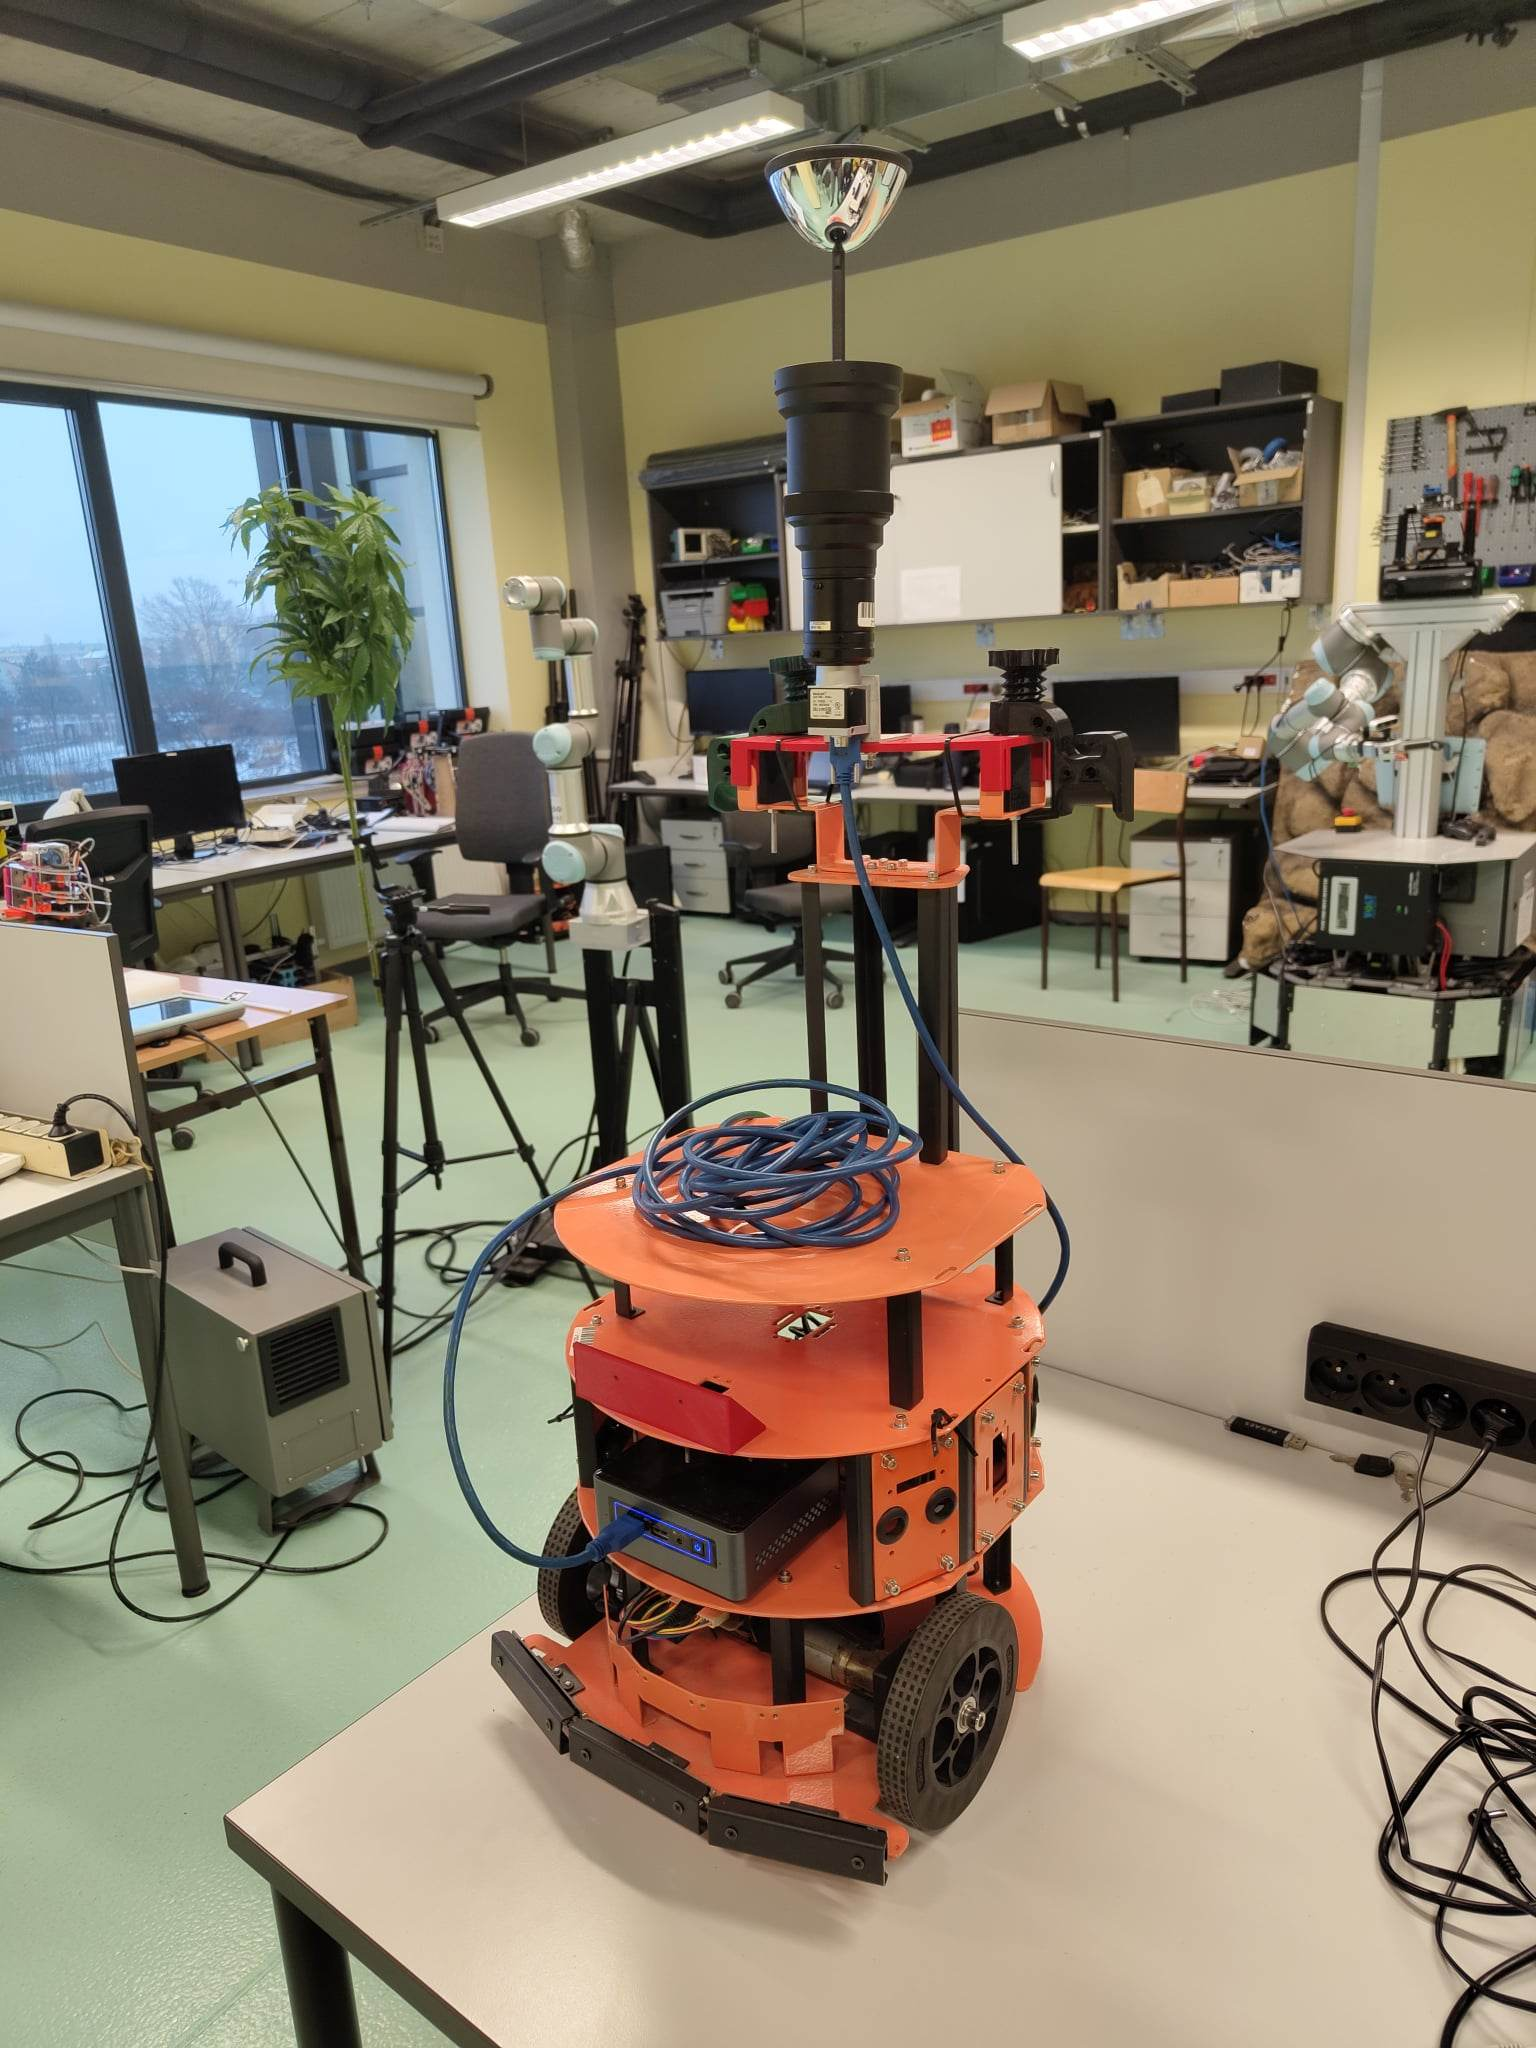
\includegraphics[scale=0.15]{Labbot&ele/2.jpg}
    \caption{LabBot-Mobile Robot}
    \label{fig:1} 
\end{figure}\
%%%%%%%%%%%%%%%%%%%%%%%%%%%%%%%%%%%%%%%%%%%%%%%%%%%%%%%%%%%


%%%%%%%%%%%%%%%%%%%%%%%%%%%%%%%%%%%%%%%%%%%%%%%%%%%%%%%%%%%%%%%%%%%%%%%%%%%%%%%%%%%%%%%%%%
\section{Tasks- Engineering work}
The following is a list of the tasks that need to be completed as part of the engineering work:
\begin{itemize}
    \item Installation of the Catadioptric sensor on the Mobile Robot (Mechanical, Electrical design and Assembly)
    \item Calibration of the Camera sensor for better input of catadioptric images.
    \item Implementation of the ROS node and the acquisition of the images from the catadioptric camera.
    \item Implementation of a selected obstacle avoidance method on the basis of the omnidirectional images.
    \item Execution of the Object Recognition added feature to the robot to understand it more efficiently.
    \item Testing and evaluation of the completed system.
\end{itemize}
%%%%%%%%%%%%%%%%%%%%%%%%%%%%%%%%%%%%%%%%%%%%%%%%%%%%%%%%%%%%%%%%%%%%%%%%%%%%%%%%%%%%%%%%%%

\section{Next Chapters Description}
The project's theoretical background is covered in the second chapter of this dissertation. The third chapter goes into further detail on how the project makes use of the theoretical knowledge. The fourth chapter concludes this essay by summarizing it.
%%%%%%%%%%%%%%%%%%%%%%%%%%%%%%%%%%%%%%%%%%%%%%%%%%%%%%%%%%%%%%%%%%%%%%%%%%%%%%%%%%%%%%%%%%%%%%%%%%%%%%%%%
%%%%%%%%%%%%%%%%%%%%%%%%%%%%%%%%%%%%%%%%%%%%%%%%%%%%%%%%%%%%%%%%%%%%%%%%%%%%%%%%%%%%%%%%%%%%%%%%%%%%%%%%%
\chapter{Theoretical knowledge}
%%%%%%%%%%%%%%%%%%%%%%%%%%%%%%%%%%%%%%%%%%%%%%%%%%%%%%%%%%%%%%%%%%%%%%%%%%%%%%%%%%%%%%%%%%%%%%%%%%%%%%%%%
\section{Camera Module}
\subsection{Besler-Camera Sensor}
The Basler acA1440-220uc USB 3.0 camera with the Sony IMX273 CMOS sensor has a maximum frame rate of 227 frames per second and a resolution of 1.6 MP.\cite{maghami2021automated}
%%%%%%%%%%%%%%%%%%%%%%%%%%%%%%%%%%%%%%%%%%%%%%%%%%%%%%%%%%%
\begin{figure}[H]
    \centering
    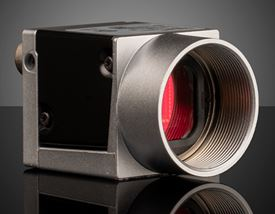
\includegraphics[scale=0.5]{Labbot&ele/3.jpg}
    \caption{Basler acA1440-220uc}
    \label{fig:Camera}
\end{figure}\
%%%%%%%%%%%%%%%%%%%%%%%%%%%%%%%%%%%%%%%%%%%%%%%%%%%%%%%%%%%
\subsection{Lens- 0-360$^{o}$}
The 0-360 Panoramic Optic is a lens attachment with an innovative optical reflector that takes a full 360-degree panorama in a single picture. The adapter is intended for use with cameras that support threaded lens attachments. 
\begin{figure}[H]
    \centering
    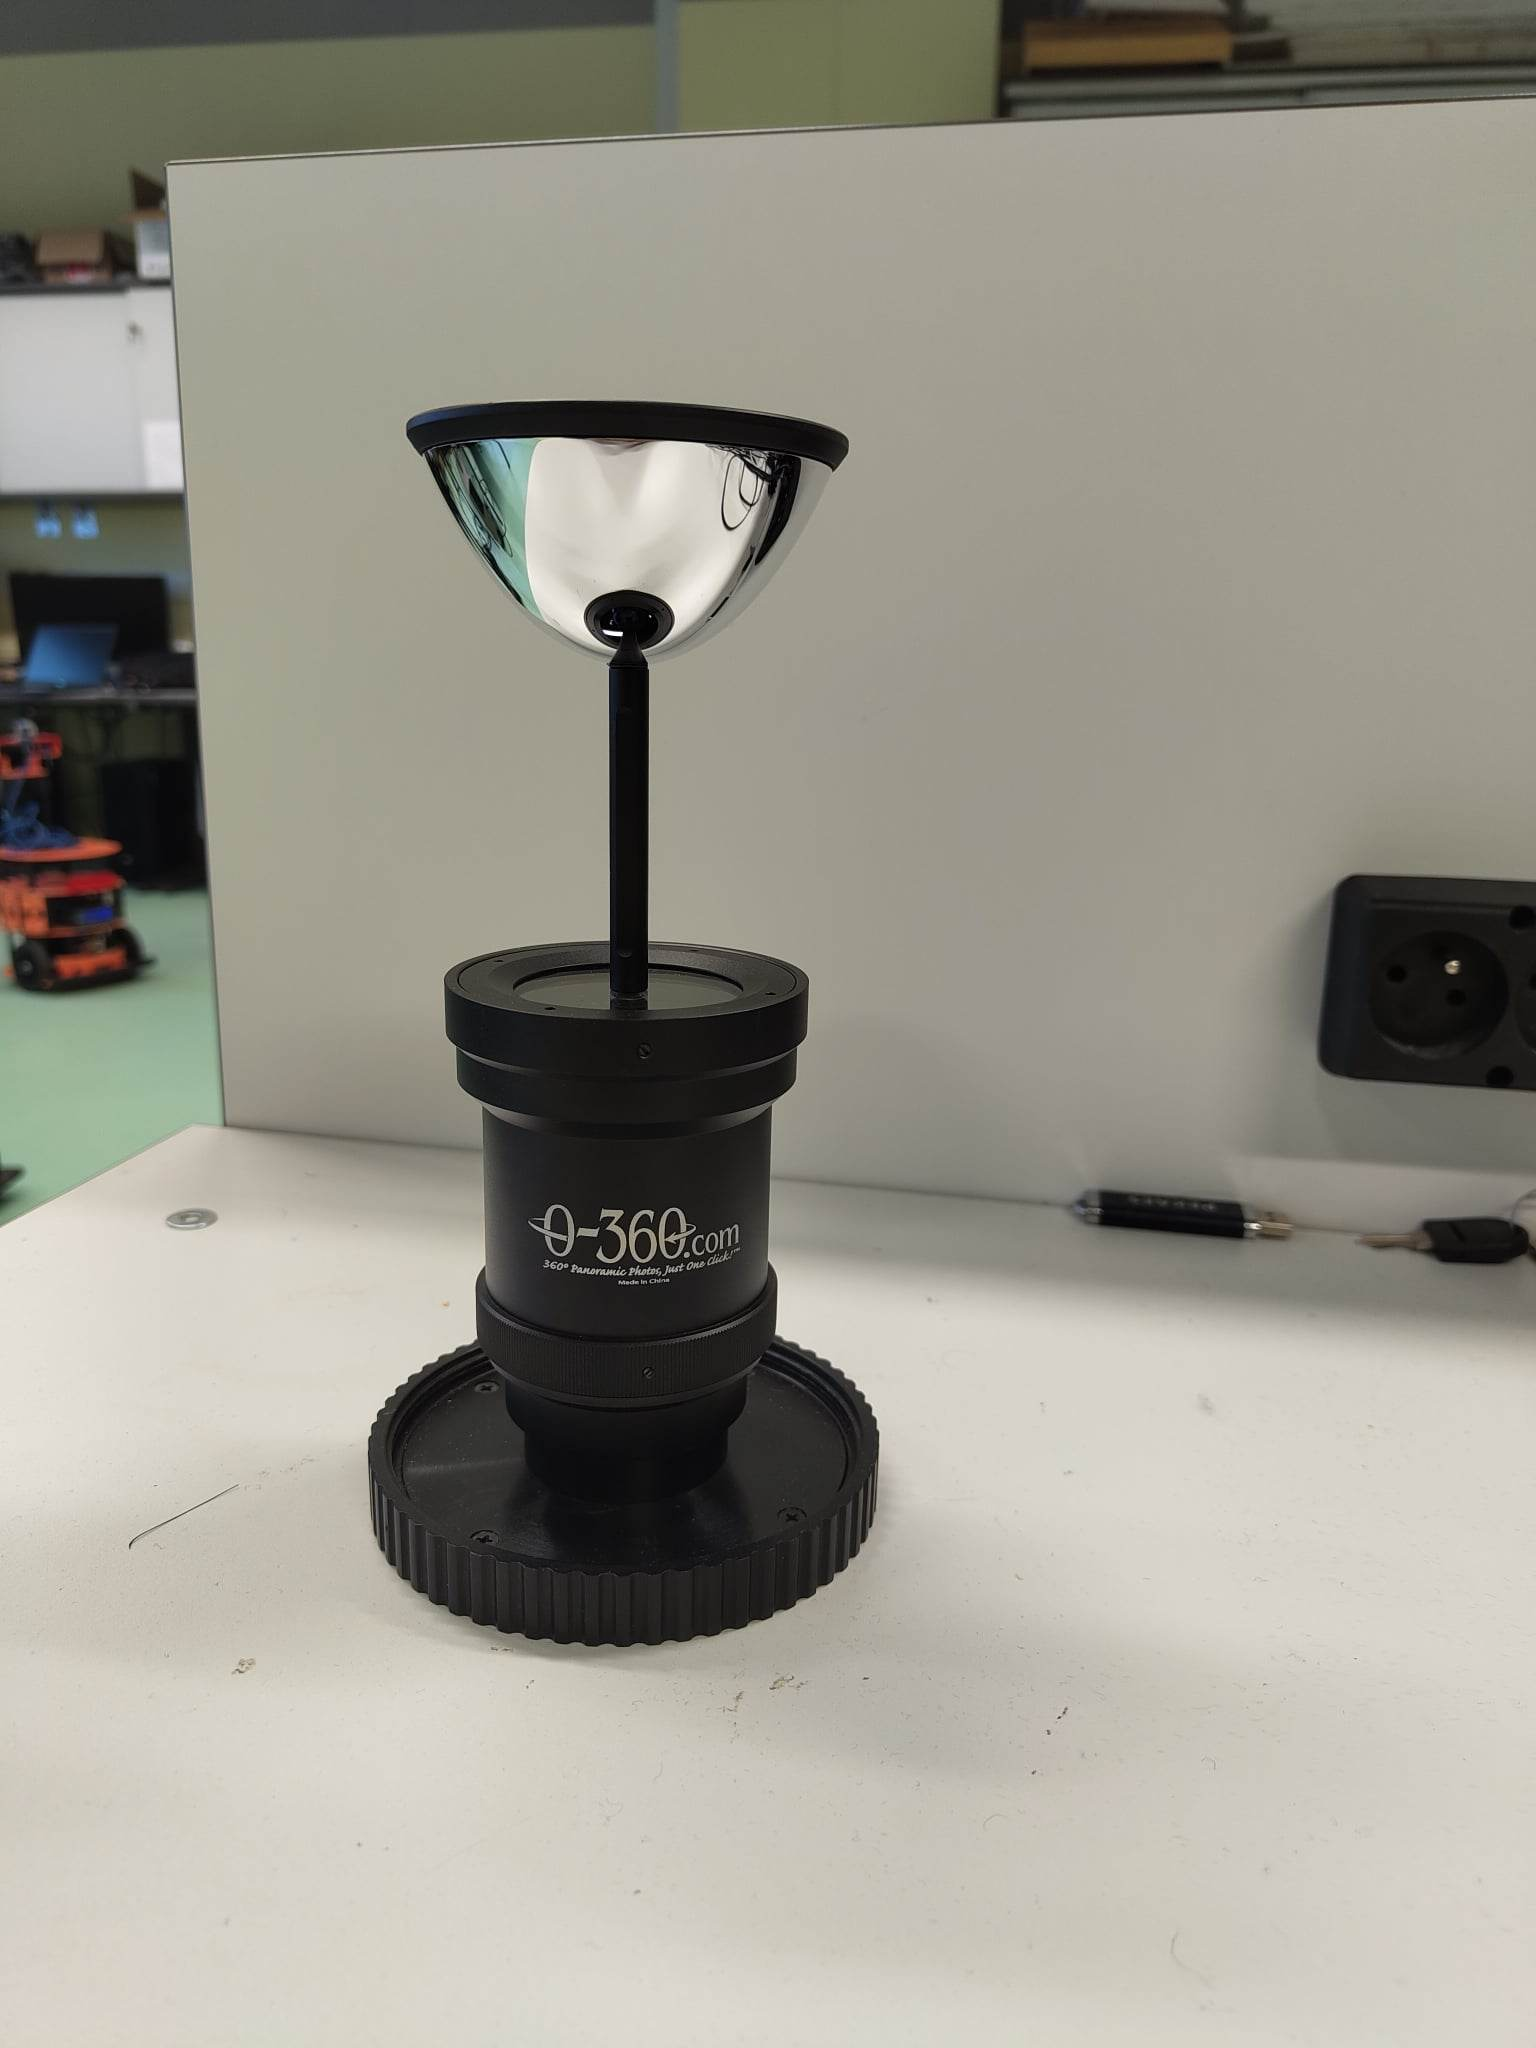
\includegraphics[scale=0.09]{Labbot&ele/4.jpg}
    \caption{0-360 Panoramic Optic–360 Degree Camera Lens}
    \label{fig:Camera}
\end{figure}\
%%%%%%%%%%%%%%%%%%%%%%%%%%%%%%%%%%%%%%%%%%%%%%%%%%%%%%%%%%%%%%%%%%%%%%%%%%%%%%%%%%%%%%%%%%%%%%%%%%%%%%%%%

%%%%%%%%%%%%%%%%%%%%%%%%%%%%%%%%%%%%%%%%%%%%%%%%%%%%%%%%%%%%%%%%%%%%%%%%%%%%%%%%%%%%%%%%%%%%%%%%%%%%%%%%%
\subsubsection{Catadioptric imaging system or Omnidirectional imaging system}
A catadioptric imaging system is a type of imaging system that uses a combination of lenses and mirrors to capture images. This type of system is often used in telescope and camera designs, as it allows for a wider field of view and a more compact design.
\newline
An Omnidirectional imaging system is a type of imaging system that can capture images in all directions. This is typically achieved through the use of multiple cameras or a single camera with a fish-eye lens. Omnidirectional imaging systems are commonly used in robotics, for example, in self-driving cars, drones, and robots for mapping and navigation.
Both Catadioptric imaging system and Omnidirectional imaging system have their own advantages and disadvantages, and the choice of which one to use depends on the specific application and the requirements.
A mechanism that achieves focal power through both reflection and refraction. While the relative powers of the lenses and mirrors vary from system to system, using reflecting surfaces to accomplish the majority of the power in conjunction with refractive surfaces with little or no power results in a picture with enhanced aberrational characteristics.
~\cite{swaminathan2007focus}. \\
To begin, we must understand the mechanics of light pathways while photographing using Fish-eye lenses. I looked around the web and discovered that the light routes look like the image below.
The blue and red points have the same (theta), thus if we know the distance of the points from the center of each plane, we can compute the x / y position.\newline
\begin{figure}[H]
    \centering
    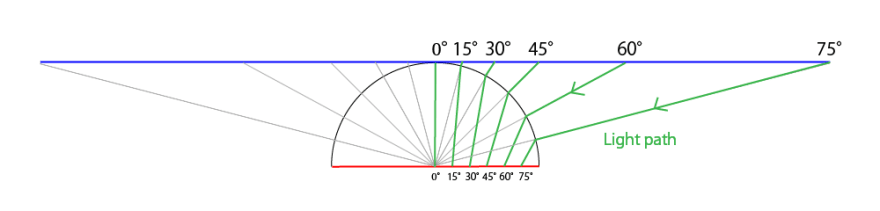
\includegraphics[scale=0.5]{Labbot&ele/5.png}
    \caption{Fish eye-Ray Diagram~\cite{bettonvil2005fisheye}}
    \label{fig:ray}
\end{figure}\
This is how the blue point will look.
$$
(x, y)=(R \tan (\varphi) \cos (\theta), R \tan (\varphi) \sin (\theta))
$$
This is how the red point will look.
$$
\left(x^{\prime}, y^{\prime}\right)=\left(\frac{2 R \varphi}{\pi} \cos (\theta), \frac{2 R \varphi}{\pi} \sin (\theta)\right)
$$
The distance of the blue point from its horizontal plane ( $r$ ) is
$$
r=\sqrt{x^2+y^2}
$$
The cosine and sine of $\theta$ are
$$
(\cos (\theta), \sin (\theta))=\left(\frac{x}{r}, \frac{y}{r}\right)
$$
The $\varphi$ is
$$
\varphi=\arctan \left(\frac{r}{R}\right)=\arctan \left(\frac{\sqrt{x^2+y^2}}{R}\right)
$$

\begin{equation}
f_{D}=\frac{2 \times V_{r} \times f}{C}=\frac{2 \times V_{r}}{\lambda} ~\cite{bettonvil2005fisheye}
\end{equation}
%%%%%%%%%%%%%%%%%%%%%%%%%%%%%%%%%%%%%%%%%%%%%%%%%%%%%%%%%%%
\begin{figure}[H]
  \centering
  \begin{minipage}[b]{0.4\textwidth}
  \begin{center}
    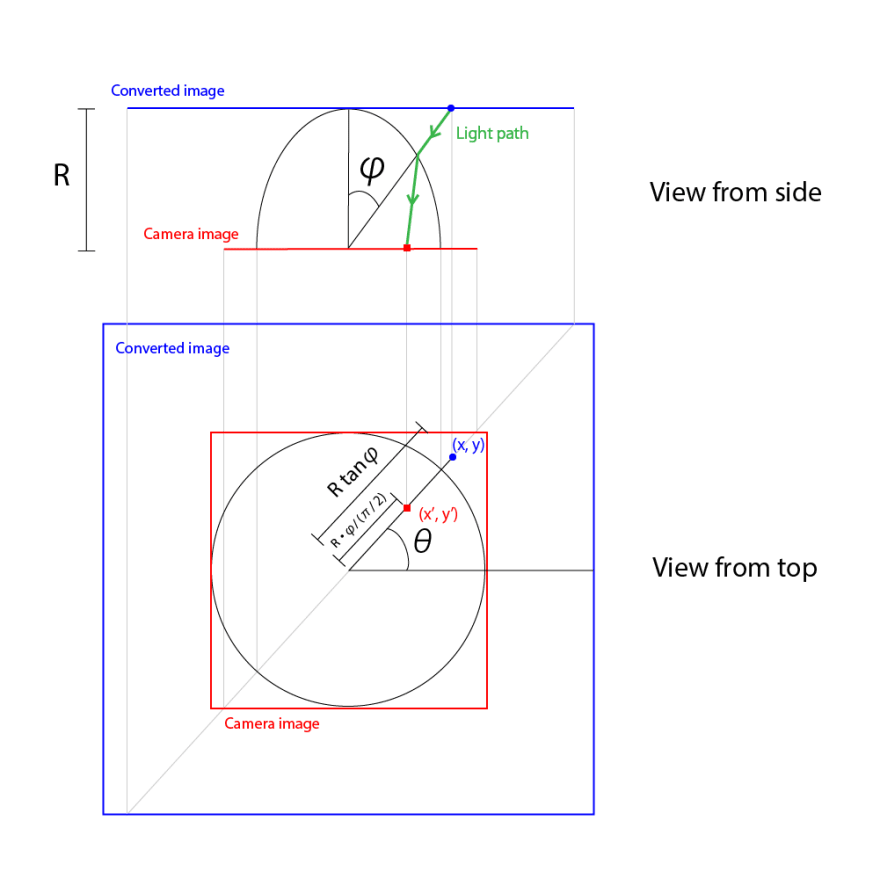
\includegraphics[scale=0.3]{Labbot&ele/6.png}
    \caption{Ray Diagram-Top and side~\cite{bettonvil2005fisheye}}
    \label{fig:ray2} 
      \end{center}
  \end{minipage}
  \hfill
  \begin{minipage}[b]{0.4\textwidth}
  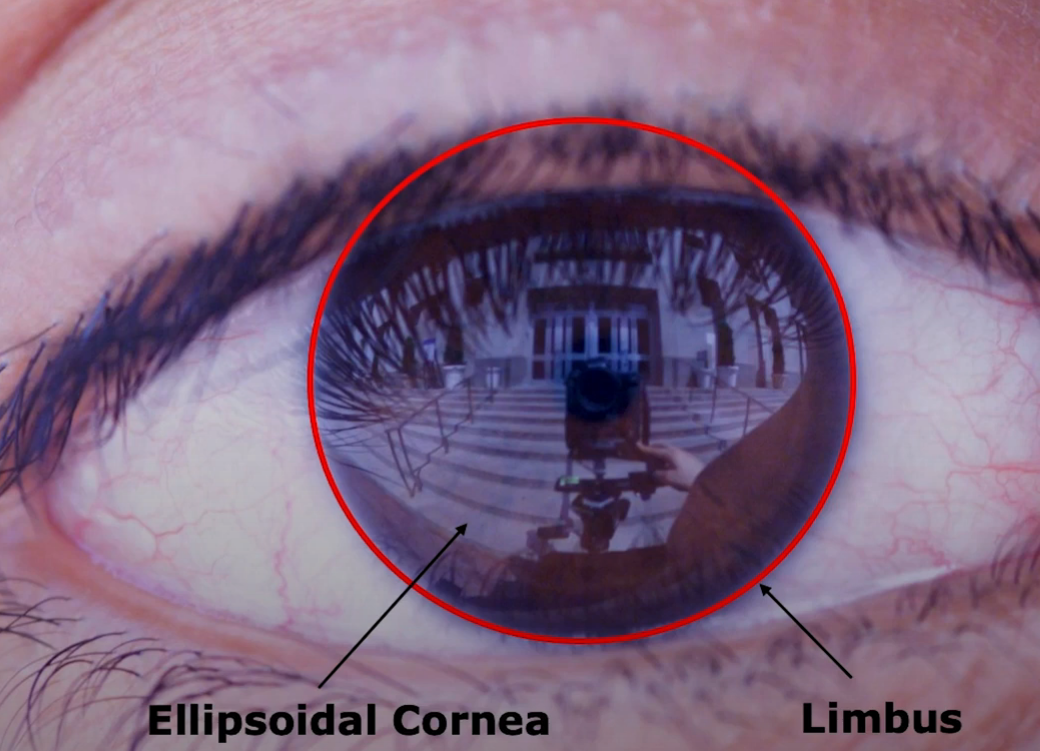
\includegraphics[scale=0.3]{Labbot&ele/7.png}
    \caption{Human eye-A working vision system}
    \label{fig:ray3} 
  \end{minipage}
\end{figure}

%%%%%%%%%%%%%%%%%%%%%%%%%%%%%%%%%%%%%%%%%%%%%%%%%%%%%%%%%%%%%%%%%%%%%%%%%%%%%%%%%%%%%%%%%%%%%%%%%%%%%%%%%

%%%%%%%%%%%%%%%%%%%%%%%%%%%%%%%%%%%%%%%%%%%%%%%%%%%%%%%%%%%%%%%%%%%%%%%%%%%%%%%%%%%%%%%%%%%%%%%%%%%%%%%%%


\chapter{Concept of the work}
This chapter will explain the project work that has been completed. We will gather all of the necessary information on the software and hardware used in the project, as well as describe the variables we considered when creating it and the problems we experienced along the way. The ultimate conclusion of the project will be discovered at the end of this chapter.

%%%%%%%%%%%%%%%%%%%%%%%%%%%%%%%%%%%%%%%%%%%%%%%%%%%%%%%%%%%%%%%%%%%%%%%%%%%%%%%%%%%%%%%%%%%%%%%%%%%%%%%%%
\section{Installations of the Catadioptric Vision System} \label{selection}
Catadioptric vision systems are found in a wide range of applications, including:
\begin{itemize}
\item Surveillance and security systems: Catadioptric cameras have a wide field of vision and are used to monitor large regions. They're common in public places like airports, train stations, and shopping malls.
\item Catadioptric cameras are used in advanced driver assistance systems (ADAS) in cars and trucks to give the driver with a wide field of view. Lane departure warning, blind spot recognition, and park assist systems are examples of this.
\item Robotics and drones: Catadioptric cameras are used for navigation, mapping, and obstacle avoidance in drones and robots. They have a large field of view, which is useful for navigating in unfamiliar environments.
\item Astronomy use catadioptric telescopes to study distant celestial objects. Because of their small size and wide field of view, they are popular among amateur astronomers.
\item Sports broadcasters utilize catadioptric cameras to capture wide-angle pictures of the field of play. They are especially effective for catching activity near the sidelines or in the corners of the field.
\item Catadioptric cameras can be used in surveying to acquire wide-angle images of the survey region. They may be used to generate detailed maps and 3D models of enormous areas.\cite{zhang2012automatic}
\end{itemize}
%%%%%%%%%%%%%%%%%%%%%%%%%%%%%%%%%%%%%%%%%%%%%%%%%%%%%%%%%%%
 \subsection{3D- Printed Mount for the camera }
 Due to availability of a solid 3-d printed platform, I used existing 3-d printed platform to install Camera sensor using the mechanical tools and the equipment which was available in the lab at that time.
\begin{figure}[H]
    \centering
    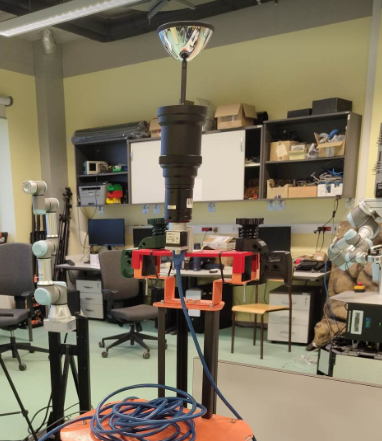
\includegraphics[scale=0.8]{Labbot&ele/3-d.png}
    \caption{Mounted Camera Module on LabBot}
    \label{fig:Platform} 
\end{figure}\

%%%%%%%%%%%%%%%%%%%%%%%%%%%%%%%%%%%%%%%%%%%%%%%%%%%%%%%%%%%%%%%%%%%%%%%%%%%%%%%%%%%%%%%%%%%%%%%%%%%%%%%%%
\subsection{Stability of the camera and the lens- Weight Differentials} 
After the motion testing of the robot with the camera module. I understand Robot made of light metal which is not stable for taking images while going at a speed of 5km/h. To overcome this issue, I took inspiration from my 3-d printed clamp-stand and I used 3-d Printed Mount/Clamps which stabilize the lens and reduce the shake effect while driving the robot at 5 km/h.

\begin{figure}[H]
  \centering
  \begin{minipage}[b]{0.4\textwidth}
  \begin{center}
    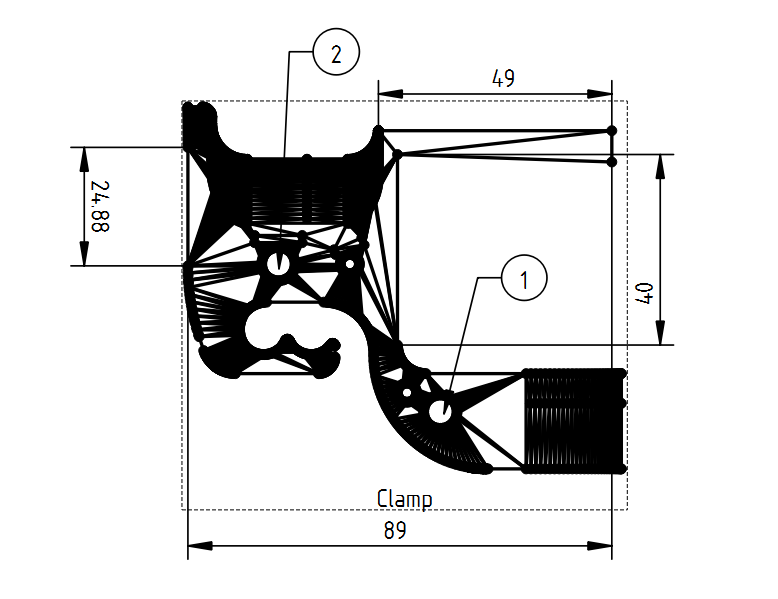
\includegraphics[scale=0.43]{Labbot&ele/n1.png}
    \caption{CAD Drawing-Clamp\cite{Github}}
    \label{fig:CAD1} 
      \end{center}
  \end{minipage}
  \hfill
  \begin{minipage}[b]{0.4\textwidth}
  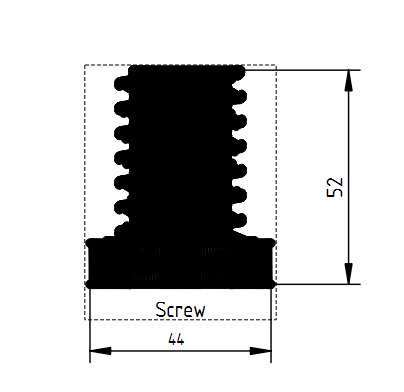
\includegraphics[scale=0.45]{Labbot&ele/n2.png}
    \caption{CAD Drawing-Screw \cite{Github}}
    \label{fig:CAD2} 
  \end{minipage}
\end{figure}

%%%%%%%%%%%%%%%%%%%%%%%%%%%%%%%%%%%%%%%%%%%%%%%%%%%%%%%%%%%
\begin{figure}[H]
  \centering
  \begin{minipage}[b]{0.4\textwidth}
  \begin{center}
    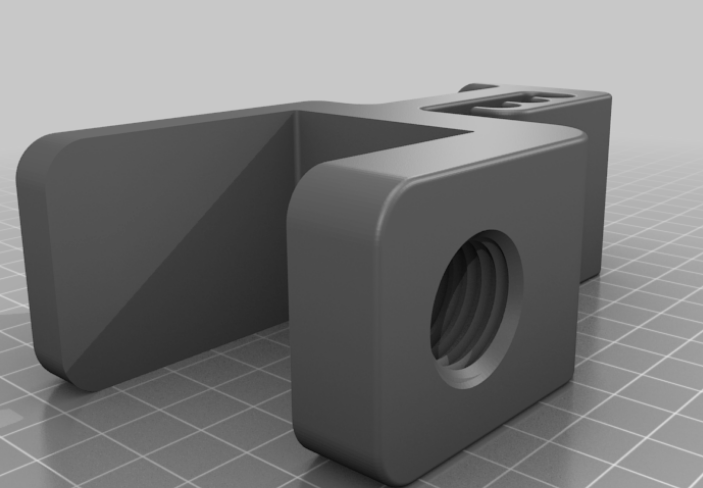
\includegraphics[scale=0.32]{Labbot&ele/3-d1.png}
    \caption{3-d Printed Clamp\cite{Github}}
    \label{fig:3d} 
      \end{center}
  \end{minipage}
  \hfill
  \begin{minipage}[b]{0.4\textwidth}
  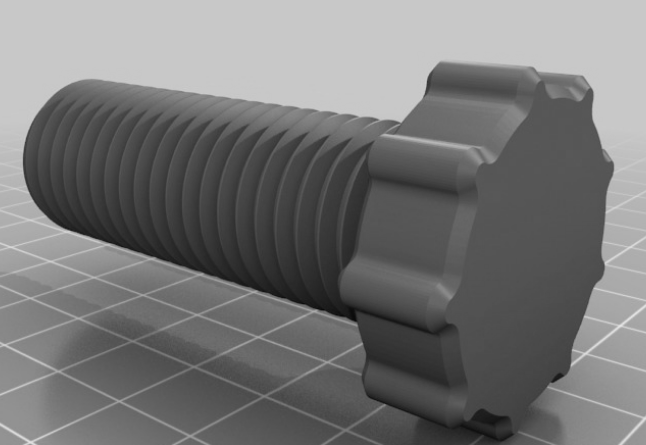
\includegraphics[scale=0.35]{Labbot&ele/3-d2.png}
    \caption{3-d Printed screw \cite{Github}}
    \label{fig:OSinter} 
  \end{minipage}
\end{figure}



%%%%%%%%%%%%%%%%%%%%%%%%%%%%%%%%%%%%%%%%%%%%%%%%%%%%%%%%%%%%%%%%%%%%%%%%%%%%%%%%%%%%%%%%%%%%%%%%%%%%%%%%%
\subsection{Calibration and Testing Stability}
Calibrating a lens on a robot entails changing the lens's focus and alignment to ensure that the pictures it collects are clear and correct. This procedure can be carried out manually by adjusting the lens by hand, or it can be carried out automatically by utilizing specialized software and algorithms. Some popular methods of lens calibration include employing a calibration target, such as a checkerboard pattern, or taking photos of a known object and determining the lens characteristics using image processing techniques. The approach employed will be determined by the type of robot and camera used.For out specific camera sensor and lens, We used Besler's- Pylon Software for the Calibration and the testing. \newline
In the below images, you can see the ball in the inner circle which is situated on top of the lens to give us an idea about the stability of the lens and the sensor. If the ball stays in inner circle in the middle, it means the lens and the sensor is stable enough to be counted as a working module.
%%%%%%%%%%%%%%%%%%%%%%%%%%%%%%%%%%%%%%%%%%%%%%%%%%%%%%%%%%%
\begin{figure}[H]
  \centering
  \begin{minipage}[b]{0.4\textwidth}
  \begin{center}
    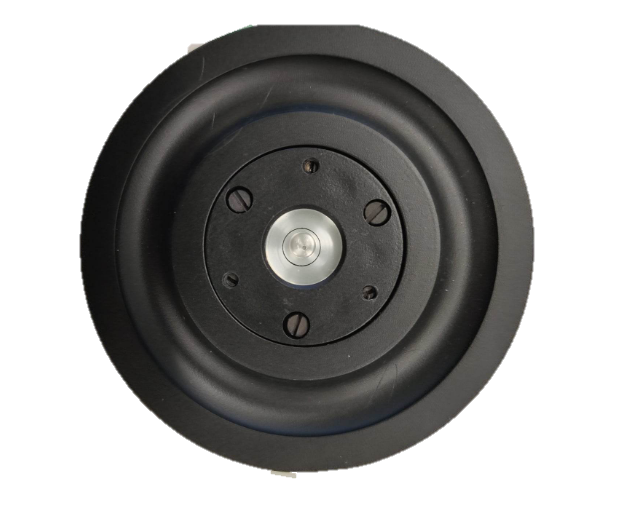
\includegraphics[scale=0.5]{Labbot&ele/o10.png}
    \caption{Stability indicator}
    \label{fig:stability}  
      \end{center}
  \end{minipage}
  \hfill
  \begin{minipage}[b]{0.4\textwidth}
    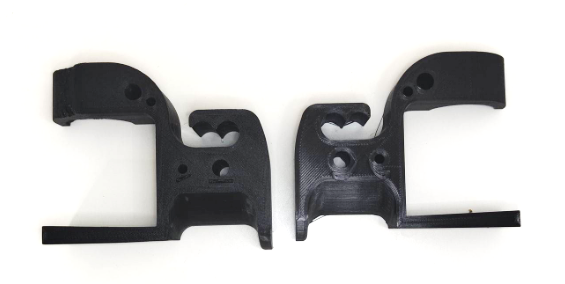
\includegraphics[scale=0.6]{Labbot&ele/qp1.png}
    \caption{3-D Printed Solution}
    \label{fig:stability}  
  \end{minipage}
\end{figure}

%%%%%%%%%%%%%%%%%%%%%%%%%%%%%%%%%%%%%%%%%%%%%%%%%%%%%%%%%%%%%%%%%%%%%%%%%%%%%%%%%%%%%%%%%%%%%%%%%%%%%%%%%
\begin{figure}[H]
    \centering
    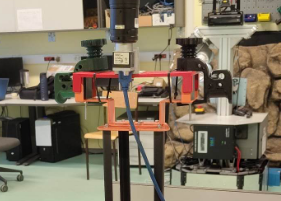
\includegraphics[scale=0.9]{Labbot&ele/19.png}
    \caption{Stable Calibration of the lens on a flat surface}
    \label{fig:output} 
\end{figure}\
\subsection{Testing the sensory images} \label{PCmini}
RGB, which stands for Red, Green, and Blue, is a color model that is used to represent and display pictures. Testing an image sensor's RGB performance entails determining the sensor's capacity to collect and reproduce colors in the red, green, and blue color channels. This can be accomplished by comparing the sensor's output to a known standard or by analyzing the sensor's color response using specialized software and algorithms. Color accuracy, color sensitivity, and color uniformity are some frequent RGB performance assessments. It's worth noting that these tests are often performed under controlled illumination conditions and with a predefined target/reference to evaluate sensor performance.

%%%%%%%%%%%%%%%%%%%%%%%%%%%%%%%%%%%%%%%%%%%%%%%%%%%%%%%%%%%
\begin{figure}[H]
    \centering
    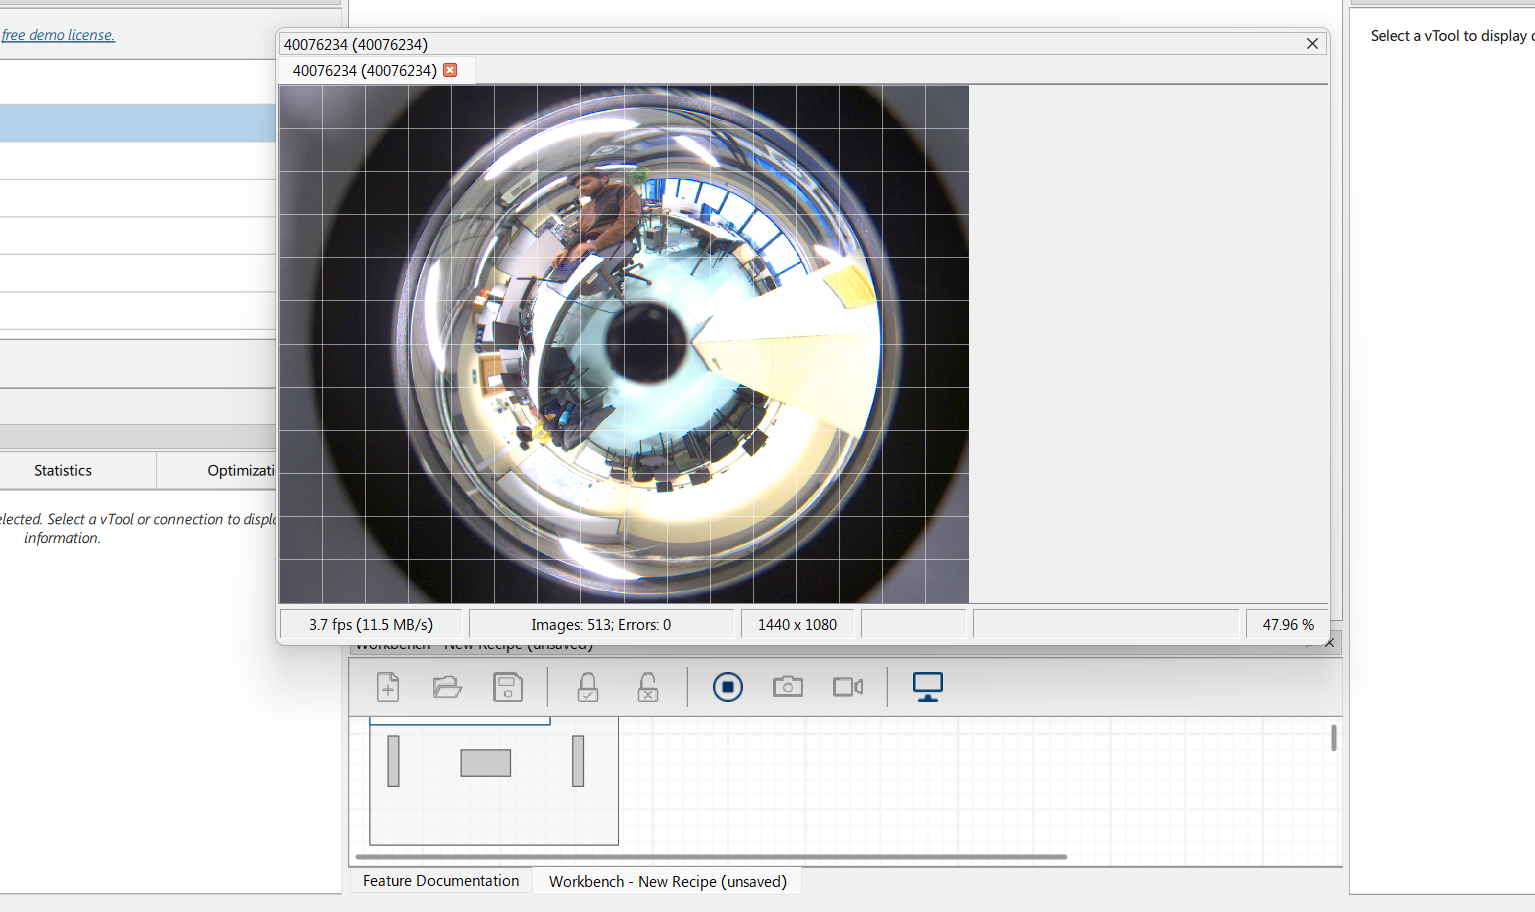
\includegraphics[scale=0.5]{Labbot&ele/11.png}
    \caption{Catadioptric image output}
    \label{fig:output} 
\end{figure}\
%%%%%%%%%%%%%%%%%%%%%%%%%%%%%%%%%%%%%%%%%%%%%%%%%%%%%%%%%%%
\begin{figure}[H]
    \centering
    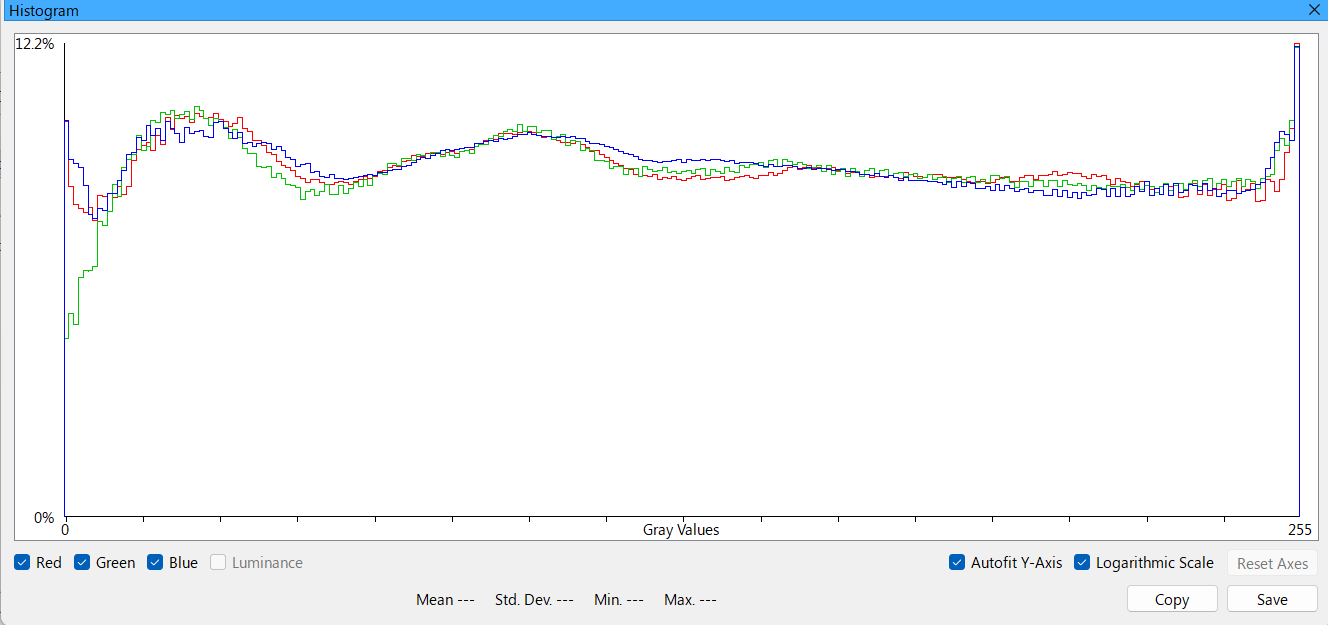
\includegraphics[scale=0.6]{Labbot&ele/12.png}
    \caption{RGB-Sensor Performance}
    \label{fig:RGB} 
\end{figure}
By displaying the distribution of gray values in the image, Plot enables you to immediately assess the quality of your image.\newline
The number of pixels per gray value is displayed on the graph.\newline
The gray values are represented on the X-axis, which runs from 0 to the greatest gray value. The chosen pixel format determines the maximum gray value.\newline
The percentage of pixels in the image that have that specific gray value is shown on the Y-axis.\newline


%%%%%%%%%%%%%%%%%%%%%%%%%%%%%%%%%%%%%%%%%%%%%%%%%%%%%%%%%%%%%%%%%%%%%%%%%%%%%%%%%%%%%%%%%%%%%%%%%%%%%%%%%
\section{Software and Environment Selection} 
\subsection{Linux}
Linux is a free and open-source operating system built on the Unix platform. It is often used in servers, desktop computers, cellphones, and embedded devices. Linux is well-known for its dependability, security, and adaptability. It may be tailored to fit the individual requirements of various users and organizations. Because Linux is designed on a modular architecture, users may select which components and functionalities to incorporate in their system. This simplifies the development of a lightweight and efficient system for a certain purpose. Linux is also extremely adaptable, with a plethora of tools and utilities at the user's disposal to change and expand the system. This indicates that its source code is freely available, allowing it to be modified and used.~\cite{thomas2006beginning}
%%%%%%%%%%%%%%%%%%%%%%%%%%%%%%%%%%%%%%%%%%%%%%%%%%%%%%%%%%%%%%%%%%%%%%%%%%%%%%%%%%%%%%%%%%%%%%%%%%%%%%%%%
\subsection{Ubuntu}
Ubuntu is a well-known Linux distribution based on Debian. It is well-known for its ease of use and user-friendliness, making it a popular choice for both desktop and server contexts. Canoncial, a UK-based firm, develops and maintains Ubuntu, and new versions are issued on a regular basis, with new versions generally released every six months. Ubuntu comes in several flavors, including a desktop version for personal computers, a server version for servers, and a mobile version for smartphones and tablets. Ubuntu comes in a variety of versions, including Kubuntu (KDE), Xubuntu (Xfce), Lubuntu (LXDE), and others. The Ubuntu user community is vast and active, and it offers assistance, documentation, and software repositories.~\cite{wei2016rt}
%%%%%%%%%%%%%%%%%%%%%%%%%%%%%%%%%%%%%%%%%%%%%%%%%%%%%%%%%%%%%%%%%%%%%%%%%%%%%%%%%%%%%%%%%%%%%%%%%%%%%%%%%
\subsection{Robot Operating System-ROS}
 ROS (Robot Operating System) is an open-source software framework that allows you to program robots. It includes a suite of frameworks and tools that enable developers to build and operate robotic systems. ROS is modular and extendable, making it simple to add new capabilities to a robot. It also offers a standardized mechanism for different sections of a robot, such as sensors, actuators, and control systems, to communicate with one another.
 \newline
 %%%%%%%%%%%%%%%%%%%%%%%%%%%%%%%%%%%%%%%%%%%%%%%%%%%%%%%%%%%%%%%%%%%%%%%%%%%%%%%%%%%%%%%%%%%%%%%%%%%%%%%%%
 ROS has several aspects that make it suitable for robotics development:
 \begin{itemize}
 \item It includes several libraries for typical robotic operations as sensor processing, navigation, and control.
\item It communicates using a message-passing paradigm, which makes it simple to add additional sensors or actuators to a robot without altering the existing code.
\item It has a huge and active community that offers assistance and adds new libraries and tools.
\item ROS is platform-agnostic and works on a wide range of operating systems, including Linux and Windows.
\item ROS is extensively used in academia and industry for robotic system research and development, and it is backed by numerous robotic businesses, including Bosch, Toyota, and Intel.
 \end{itemize}
%%%%%%%%%%%%%%%%%%%%%%%%%%%%%%%%%%%%%%%%%%%%%%%%%%%%%%%%%%%
\subsection{VMware Workstation}
VMware Workstation has several features that make it valuable for developers and IT professionals, including:
 \begin{itemize}
        \item It is compatible with a variety of operating systems, including Windows, Linux, and MacOS.
        \item It enables users to establish and maintain virtual networks, which enable virtual computers to interact with one    another as if they were on a real network.
        \item It has an easy-to-use interface for building, configuring, and maintaining virtual machines.
        \item It enables users to create virtual machine snapshots, which may then be used to swiftly restore a computer to a prior 
         condition.
        \item It integrates with VMware vSphere and vCloud, allowing for the management of virtualized environments, as well as live transfer of virtual machines across host systems.
 \end{itemize}
 %%%%%%%%%%%%%%%%%%%%%%%%%%%%%%%%%%%%%%%%%%%%%%%%%%%%%%%%%%%%%%%%%%%%%%%%%%%%%%%%%%%%%%%%%%%%%%%%%%%%%%%%%
 \begin{figure}[H]
\centering
   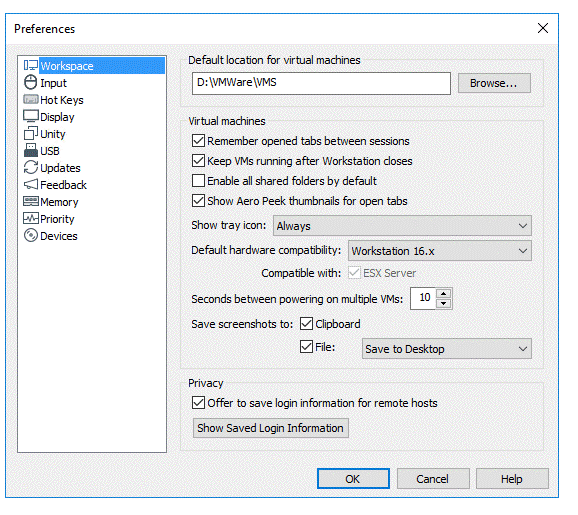
\includegraphics[scale=0.6]{Labbot&ele/vmware.png}
    \caption{VMware Workstation}
    \label{fig:VMware Workstation}
\end{figure}\
%%%%%%%%%%%%%%%%%%%%%%%%%%%%%%%%%%%%%%%%%%%%%%%%%%%%%%%%%%%%%%%%%%%%%%%%%%%%%%%%%%%%%%%%%%%%%%%%%%%%%%%%%
\subsection{Workspaces}
A catkin workspace is a sort of workspace that is used to create ROS (Robot Operating System) packages. It is a folder structure containing the source code and build files for one or more ROS packages. This directory structure is used by the catkin build system, which is the official build system for ROS, to produce and manage packages.

A catkin workspace's basic structure contains the following directories:
 \begin{itemize}
\item src: includes the source code for the ROS packages in the workspace.
\item build: stores the catkin build system's build files and artifacts.
\item devel: includes the built packages as well as additional artifacts required to execute and test the packages.
 \end{itemize}
%%%%%%%%%%%%%%%%%%%%%%%%%%%%%%%%%%%%%%%%%%%%%%%%%%%%%%%%%%%%%%%%%%%%%%%%%%%%%%%%%%%%%%%%%%%%%%%%%%%%%%%%%
%%%%%%%%%%%%%%%%%%%%%%%%%%%%%%%%%%%%%%%%%%%%%%%%%%%%%%%%%%%%%%%%%%%%%%%%%%%%%%%%%%%%%%%%%%%%%%%%%%%%%%%%%
\subsection{ROS-Package and Topic}
A package is a software organization unit. It can include a node, a standalone library, a data collection, or anything else that constitutes a standalone module. The primary goal of the packages is to allow for the simple and reuse usage of previously written applications.\newline
A topic is a type of bus on which nodes communicate with one another. Each topic must have a distinct name and a distinct category. The node receiving data from the subject (subscriber) is ignorant of its existence and is unable to identify the node publishing the data, and vice versa. Under one topic, there may be several publishers and subscribers. \newline


%%%%%%%%%%%%%%%%%%%%%%%%%%%%%%%%%%%%%%%%%%%%%%%%%%%%%%%%%%%%%%%%%%%%%%%%%%%%%%%%%%%%%%%%%%%%%%%%%%%%%%%%%
\subsection{ROS- Bag and Service}
A ROS bag (short for "log") is a file type that is used in ROS to record and replay data (Robot Operating System). A ROS bag is a file that includes one or more streams of data from a running ROS system, such as sensor readings, pictures, or command messages. These data streams can be collected from various subjects and nodes and saved in a single bag file.
ROS bags are used for a variety of purposes, including:
\begin{itemize}
    \item Data collection from an operating robot for later study and debugging
    \item Reproducing data from a prior run in order to test and validate new software
    \item Data sharing for testing and development with other academics and developers
    \item Testing and simulation using recorded data
\end{itemize}
A ROS service is a form of inter-process communication (IPC) mechanism in ROS (Robot Operating System) that allows nodes to request and receive responses from other nodes. The request-response model is used by services, in which one node sends a request message to another node, which then executes a certain action and sends a response message back.
\newline
A service definition file, which is commonly a.srv file and contains the request and response message types, defines the service. The package and service name, which are unique across the ROS system, define services. The package and service name, which are unique across the ROS system, define services.
Services are helpful when a specified activity or operation must be completed and a response is needed, such as:
\begin{itemize}
\item Requesting a specific sensor reading
\item Requesting a robot to move to a specific location
\item Requesting a specific configuration change
\end{itemize}
%%%%%%%%%%%%%%%%%%%%%%%%%%%%%%%%%%%%%%%%%%%%%%%%%%%%%%%%%%%%%%%%%%%%%%%%%%%%%%%%%%%%%%%%%%%%%%%%%%%%%%%%%
 \subsection{ ROS Utilities}
 \subsubsection{RQT graph}
 RQT (Robot Quality Tools) is a collection of ROS (Robot Operating System) tools that provide a graphical interface for monitoring and troubleshooting a running ROS system. RQT Graph is one of RQT's tools for displaying the communication graph of an operating
 ROSsystem. It depicts the system's nodes, topics, and services, as well as how they are linked to one another.
 %%%%%%%%%%%%%%%%%%%%%%%%%%%%%%%%%%%%%%%%%%%%%%%%%%%%%%%%%%%
 \subsubsection{RQT Bag}
RQT Bag is a ROS (Robot Operating System) application developed by RQT that lets users to capture and play back data from a running ROS system. It is a graphical user interface for the command-line utility rosbag, which is used to record and playback ROS bags. RQT Bag is an easy-to-use interface for managing bag files and allows users to record, play, stop, and search through bag files.
\newline
%%%%%%%%%%%%%%%%%%%%%%%%%%%%%%%%%%%%%%%%%%%%%%%%%%%%%%%%%%%
 \subsubsection{Rviz}
RViz (Robot Operating System Visualization) is a 3D visualization tool for ROS (Robot Operating System) that allows users to display sensor data such as point clouds, laser scans, and 3D models, as well as robot status information such as the robot's attitude and trajectory. RViz is a sophisticated tool for debugging, testing, and assessing the performance of a robot.

RViz is a 3D visualization framework that is based on the famous Ogre3D library and provides a user-friendly interface for viewing a wide range of data sources. It allows users to add and customize various visualizations such as point clouds, laser scans, and 3D models, as well as show many sorts of data such as TF frames, Odometry, trajectories, and so on.
%%%%%%%%%%%%%%%%%%%%%%%%%%%%%%%%%%%%%%%%%%%%%%%%%%%%%%%%%%%
 \subsection{LabBot Package}
 This study would not have been feasible without the current software package that enhanced LabBot's capability. It was written in 2015 by two students for their engineering thesis\cite{Labbot1} and was then used in this work. It enables, among other things, control of the robot through a controller via a suitable node, which prioritizes transmitting information supplied from the controller to the controller, where it is then transferred to the wheels of the robot. This capability allowed the LabBot to be moved swiftly and effectively through the specified locations and around designated obstacles. The program also tracks the robot's current position in its coordinate system by reading and processing encoder pulses.\cite{Githublab}
%%%%%%%%%%%%%%%%%%%%%%%%%%%%%%%%%%%%%%%%%%%%%%%%%%%%%%%%%%%
\begin{figure}[H]
    \centering
    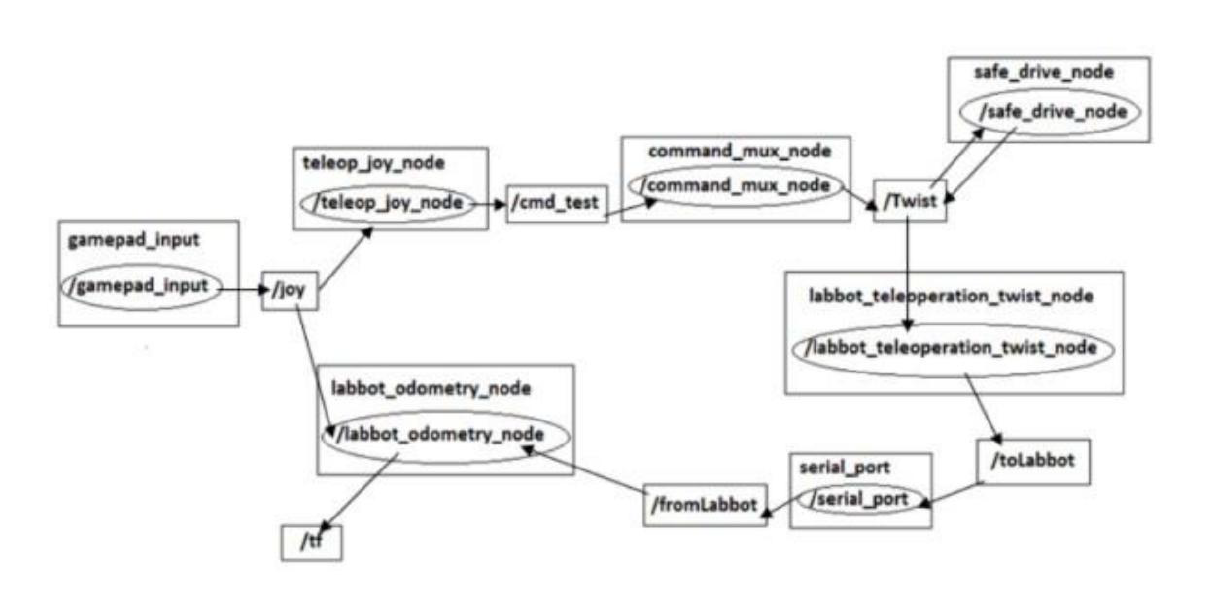
\includegraphics[scale=0.5]{Labbot&ele/14.png}
    \caption{LabBot Nodes and Topics}
    \label{fig:Package} 
\end{figure}
%%%%%%%%%%%%%%%%%%%%%%%%%%%%%%%%%%%%%%%%%%%%%%%%%%%%%%%%%%%
\subsection{Python}
A high-level, interpreted general-purpose programming language. An open-source library devoted to computer vision activities carried out in. Its leitmotif is concern for code structure and readability, which is enforced by the requirement to use indentation and tabulators (for example, when restricting the range of constant code components, such as loops, functions, and conditional instructions). Due to the necessity to comply with the machine learning library TensorFlow 2.7.0 (the version we use requires Python>=3.8.0), the language version 3.8.10 was utilized in the work.
%%%%%%%%%%%%%%%%%%%%%%%%%%%%%%%%%%%%%%%%%%%%%%%%%%%%%%%%%%%
\subsection{Open CV and TensorFlow Libraries}
OpenCV (Open Source Computer Vision Library) is a programming function library geared mostly at real-time computer vision. It is free and open-source, and it has been used in a variety of applications including object identification, image processing, video analysis, and others. It includes a wide range of image and video processing tools and functionalities, such as image filtering, feature identification, and picture segmentation. C++, Python, Java, and MATLAB are among the programming languages supported by OpenCV.~\cite{dadhich2018practical}\newline
TensorFlow is an open-source machine learning and deep learning software library. It was created by Google and is extensively used in business and academics to construct and deploy machine learning models. TensorFlow includes a variety of tools for developing and training machine learning models, including neural networks, deep learning, and reinforcement learning. It also includes a plethora of pre-trained models and libraries for applications like image classification, object identification, and natural language processing. TensorFlow supports a variety of programming languages, including Python, C++, and Java.\newline
OpenCV and TensorFlow may be used in conjunction to perform a variety of computer vision tasks such as object identification, picture classification, and semantic segmentation. The picture data can be pre-processed and organized using OpenCV, and machine learning models can be trained and deployed using TensorFlow. They can work together to create a strong and adaptable solution for computer vision problems.
\subsection{SQL Flowchart for ROS Node Image Prediction using ERFNet Interpreter}
Here we start implementing our idea in which a ROS (Robot Operating System) node that subscribes to an image topic and a string topic, processes the image with a TensorFlow Lite interpreter, saves both the processed and original images, and then sends a Twist message.

\begin{lstlisting}
                                 +--------------+
                                 | IMPORT LIBRARIES |
                                 +--------------+
                                            |
                                 +-----------------+
                                 | DEFINE CLASS "CALLBACKS" |
                                 +-----------------+
                                            |
                                 +-----------------------------+
                                 | INITIALIZE VARIABLES & OBJECTS |
                                 +-----------------------------+
                                            |
                                 +-------------------------+
                                 | SET UP SUBSCRIBERS & PUBLISHER |
                                 +-------------------------+
                                            |
                                 +---------------+
                                 | IMAGE-CALLBACK |
                                 +---------------+
                                            |
                                 +------------------------+
                                 | PROCESS METHOD (CHECK IMAGE, SAVE, MAKE PREDICTION) |
                                 +------------------------+
                                            |
                                 +--------------------------------------+
                                 | MAKE-PREDICTION METHOD (TIMER, NUMPY, INTERPRETER, PREDICTIONS, THRESHOLD, WRITE IMAGE, PRINT TIME) |
                                 +--------------------------------------+
                                            |
                                 +-----------------------------+
                                 | MAIN BLOCK (INITIALIZE ROS NODE, INSTANCE, RUN PROCESS METHOD LOOP) |
                                 +-----------------------------+
\end{lstlisting}

%%%%%%%%%%%%%%%%%%%%%%%%%%%%%%%%%%%%%%%%%%%%%%%%%%%%%%%%%%%
\begin{itemize}
\item I start by importing all the necessary libraries such as rospy, numpy, sensor-msgs, std-msgs, geometry-msgs, cv-bridge, cv2, tensorflow, time, and keras.
\item I then define a class called "Callbacks" which contains all the methods and variables I will use in the program.
\item In the init method of the Callbacks class, I initialize several variables and objects including the image, bridge, folder-path, erfnet-interpreter, erfnet-input-details, erfnet-output-details, num, and rate.
\item  I also set up subscribers for the topics "/cv-camera/image-raw" and "/speeding" and a publisher for the topic "/Twist" which I will use later on.
\item  The image-callback method is called when a new image is received on the topic "/cv-camera/image-raw", it converts the image from a ROS Image message to a cv2 image format.
\item  The process method is called in a while loop and it checks if an image is received, if it is, it saves the image to a file and calls the make-prediction method.
\item  In the make-prediction method, I first start a timer, then I convert the image to a numpy array, expand its dimensions and print its shape.
\item I then set the image as the input tensor for the erfnet-interpreter, invoke the interpreter and get the predictions from the model.
\item I then threshold the predictions, write the resulting image to a file, and print the time it took to load the image and the time it took to make the prediction.
\item  Finally, in the main block, I initialize a node for ros, create an instance of the Callbacks class, and run a while loop that calls the process method with a rate of $0.5 \mathrm{~Hz}$.\cite{Github}
\end{itemize}
%%%%%%%%%%%%%%%%%%%%%%%%%%%%%%%%%%%%%%%%%%%%%%%%%%%%%%%%%%%
\subsection{YOLO v3}
You Only Look Once (YOLO) is a real-time object recognition technique used in computer vision applications. The third iteration of the YOLO algorithm, YOLO v3, is an improvement over earlier versions.
YOLO v3 is a deep learning method that detects and classifies objects in images using a convolutional neural network (CNN). It splits an image into a grid of cells and predicts the bounding boxes and class probabilities of the items that may be present in that cell for each cell. Because it does not need to analyze the full image several times, YOLO v3 can recognize many items in an image and is quicker than other object identification methods.~\cite{redmon2018yolov3}\newline
The enhanced accuracy of YOLO v3 over earlier versions is due to a new architecture dubbed Darknet-53, which is a deeper and more powerful CNN. YOLO v3 additionally employs anchor boxes to increase the accuracy of bounding box predictions, and it offers a new approach called "intersection over union" (IOU) to measure prediction accuracy.
YOLO v3 is widely utilized in a wide range of computer vision activities, including self-driving automobiles, surveillance systems, and video analysis. It is well-known for its real-time performance and great accuracy, as well as being open-source and having a big community that offers pre-trained models, training, and assistance.

%%%%%%%%%%%%%%%%%%%%%%%%%%%%%%%%%%%%%%%%%%%%%%%%%%%%%%%%%%%
\begin{figure}[H]
    \centering
    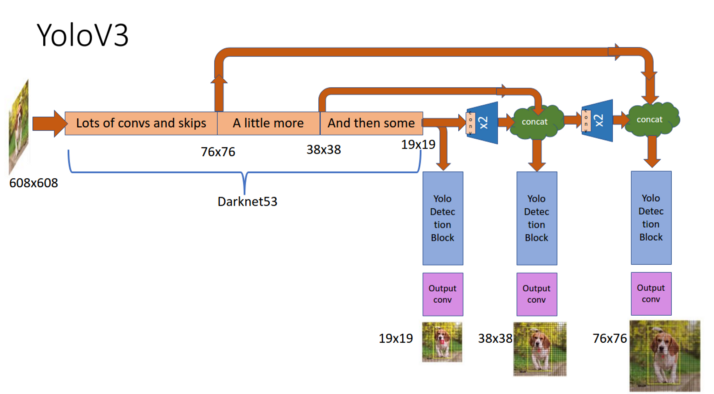
\includegraphics[scale=1.0]{Labbot&ele/w1.png}
    \caption{YOLO-V3 Architecture\cite{redmon2018yolov3}}
    \label{fig:Package} %https://towardsdatascience.com/yolo-v3-explained-ff5b850390f
\end{figure}\
%%%%%%%%%%%%%%%%%%%%%%%%%%%%%%%%%%%%%%%%%%%%%%%%%%%%%%%%%%%
\begin{figure}[H]
    \centering
    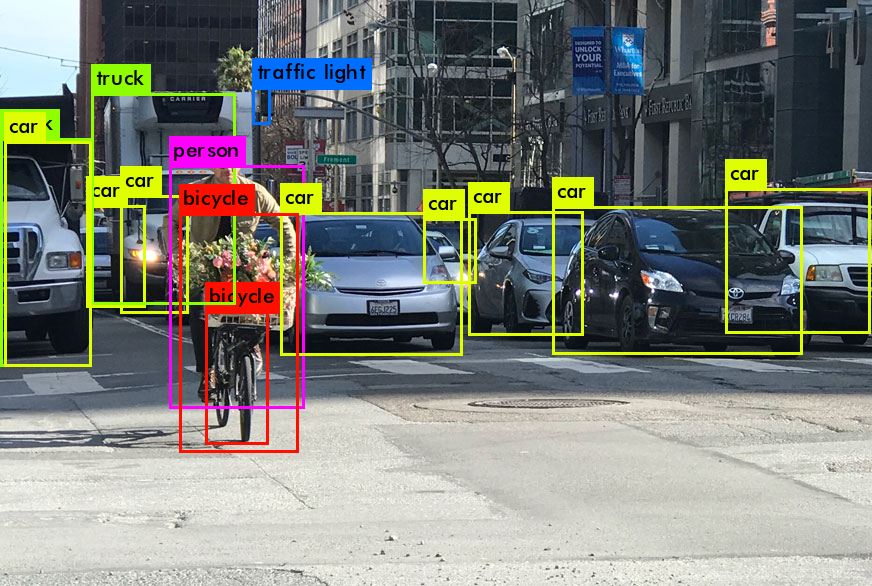
\includegraphics[scale=0.5]{Labbot&ele/o15.png}
    \caption{Example of Object Recognition using YOLO v3~\cite{Yolov3}}
    \label{fig:Package}
\end{figure}\
%%%%%%%%%%%%%%%%%%%%%%%%%%%%%%%%%%%%%%%%%%%%%%%%%%%%%%%%%%%

\subsection{SQL based Flowchart diagram to understand Object Recognition}
\begin{lstlisting}
            +-------------+      +-------------------+      +------------+
            | Import libs |------>| Initialize ROS node |------>| Load model |
            +-------------+      +-------------------+      +------------+
                                                                        |
                                                                        v
                                                             +-----------------+
                                                             | Set input size |
                                                             +-----------------+
                                                                        |
                                                                        v
                                                             +-----------------+
                                                             | Callback func  |
                                                             +-----------------+
                                                                        |
                                                                        v
                                                             +-----------------+
                                                             | Convert image  |
                                                             +-----------------+
                                                                        |
                                                                        v
                                                             +-----------------+
                                                             | Predict boxes  |
                                                             +-----------------+
                                                                        |
                                                                        v
                                                             +-----------------+
                                                             | Filter boxes   |
                                                             +-----------------+
                                                                        |
                                                                        v
                                                             +-----------------+
                                                             | Draw boxes     |
                                                             +-----------------+
                                                                        |
                                                                        v
                                                             +-----------------+
                                                             | Publish image  |
                                                             +-----------------+


\end{lstlisting}
%%%%%%%%%%%%%%%%%%%%%%%%%%%%%%%%%%%%%%%%%%%%%%%%%%%%%%%%%%%
\begin{itemize}
    \item I imported the necessary libraries such as CV2 and ROS.
  \item I initialized the ROS node to subscribe to the image topic.
  \item I loaded the pre-trained YOLOv3 model.
  \item I set the model's input size to match the size of the images being received from the ROS node.
  \item I set up a callback function to handle the incoming images from the ROS node.
  \item In the callback function, I converted the ROS image message to a format that can be processed by the model.
  \item I passed the image through the YOLOv3 model to obtain the bounding boxes and class predictions.
  \item I filtered the predictions based on a certain threshold value.
  \item I drew the bounding boxes and class labels on the image.
  \item I published the processed image back to a ROS topic for display or further processing.\cite{Github}
\end{itemize}
%%%%%%%%%%%%%%%%%%%%%%%%%%%%%%%%%%%%%%%%%%%%%%%%%%%%%%%%%%%
\subsection{Loss Function-YOLO}
YOLO (You Only Look Once) is a real-time object detection system that detects items in an image using a single convolutional neural network (CNN). The YOLO network has been trained to predict item bounding boxes and class probabilities in images. In YOLO, the loss function is a hybrid of two loss functions:~\cite{zhang2012automatic}
\begin{itemize}
\item The localization loss, which is used to train the network to predict the bounding boxes of objects in the image, is the initial loss function. This loss function is frequently implemented by calculating the mean squared error (MSE) or the smooth L1 loss between the expected and ground-truth bounding box coordinates.
\item The classification loss function is used to train the network to predict the class probabilities of objects in the image. The cross-entropy loss between predicted class probabilities and ground-truth class labels is used to create this loss function.
\end{itemize}
The total loss function is the weighted average of the localization and classification losses. To balance the trade-off between localization precision and classification accuracy, the weights on the two loss functions can be changed.
%%%%%%%%%%%%%%%%%%%%%%%%%%%%%%%%%%%%%%%%%%%%%%%%%%%%%%%%%%%
\begin{equation}
\begin{aligned}
& \lambda_{\text {coord }} \sum_{i=0}^{S^2} \sum_{j=0}^B 1_{i j}^{o b j}\left[\left(x_i-\hat{x}_i\right)^2+\left(y_i-\hat{y}_i\right)^2\right] \\
& +\lambda_{\text {coord }} \sum_{i=0}^{S^2} \sum_{j=0}^B 1_{i j}^{o b j}\left[\left(\sqrt{w_i}-\sqrt{\hat{w}_i}\right)^2+\left(\sqrt{h_i}-\sqrt{\hat{h}_i}\right)^2\right] \\
& +\sum_{i=0}^{S^2} \sum_{j=0}^B 1_{i j}^{o b j}\left(C_i-\hat{C}_i\right)^2+\lambda_{\text {noobj }} \sum_{i=0}^{S^2} \sum_{j=0}^B 1_{i j}^{n o o b j}\left(C_i-\hat{C}_i\right)^2 \\
& +\sum_{i=0}^{S^2} 1_i^{o b j} \sum_{c \in c l a s s e s}\left(p_i(c)-\hat{p}_i(c)\right)^2~ \cite{choi2018deep}
\end{aligned}
\end{equation}
%%%%%%%%%%%%%%%%%%%%%%%%%%%%%%%%%%%%%%%%%%%%%%%%%%%%%%%%%%%
The YOLO algorithm uses 3 constants, called $3 \lambda$, to balance the importance of different parts of the loss function in the model. The prediction output of the model is a vector that contains information about bounding box and class predictions for each grid cell in the image. The real value for the confidence score for each box is determined by the intersection over union of the predicted bounding box and the actual bounding box from the label. The term $1_i^{o b j}$ is used to indicate if there is an object present in a specific cell and it is equal to 1 if there is an object and 0 otherwise. The term $1_{i j}^{o b j}$ is equal to 1 when there is an object in a cell and the confidence of the $j$th predictor of that cell is the highest among all predictors for that cell.\newline
Additionally, the term $1_{i j}^{n o o b j}$ is used to indicate when there are no objects in a specific cell and it is equal to 1 when there are no objects and 0 otherwise. In other words, these terms are used to identify when an object is present or not in a specific cell, and which of the bounding box predictors for that cell is the most confident in its prediction. Overall, these terms and constants are used to help the model accurately predict the bounding boxes and class labels for objects in an image.
%%%%%%%%%%%%%%%%%%%%%%%%%%%%%%%%%%%%%%%%%%%%%%%%%%%%%%%%%%%
\subsection{COCO (Common Objects in Context)}
The Microsoft Research team generated COCO (Common Objects in Context), a large-scale picture recognition dataset. It is intended for tasks like as object detection, segmentation, keypoint detection, and captioning. The COCO dataset is frequently utilized in both computer vision research and industry.\newline
Approximately 330,000 photos are included in the collection, along with 80 item types and over 2.5 million object instances. The photographs were gathered from many sources, including the internet, and vary in terms of item scale, attitude, and scene arrangement. COCO also contains over 250,000 object segmentations and over 5 million object keypoints, making it one of the largest and most diversified datasets for object recognition, segmentation, and keypoint detection tasks.~\cite{lin2014microsoft}\newline
The COCO dataset has been utilized in a number of computer vision research articles as well as machine learning contests such as the Microsoft COCO Object Detection Challenge and the COCO Keypoints Challenge. Microsoft Research actively maintains the COCO dataset, and new pictures and annotations are contributed on a regular basis. The dataset is open to use for non-commercial purposes, and the photos and annotations are free to download.\newline
%%%%%%%%%%%%%%%%%%%%%%%%%%%%%%%%%%%%%%%%%%%%%%%%%%%%%%%%%%%

\subsection{Object Recognition Implementation using Catadioptric system}
\begin{lstlisting}
    [ROS Node]--->[Preprocess Images]--->[YOLOv3 Model]--->[Loop]
           |                                             |
           v                                             v
       [Subscribe]<---[Visualize]<---[Publish]<---[Repeat]
\end{lstlisting}
 \begin{figure}[H]
    \centering
    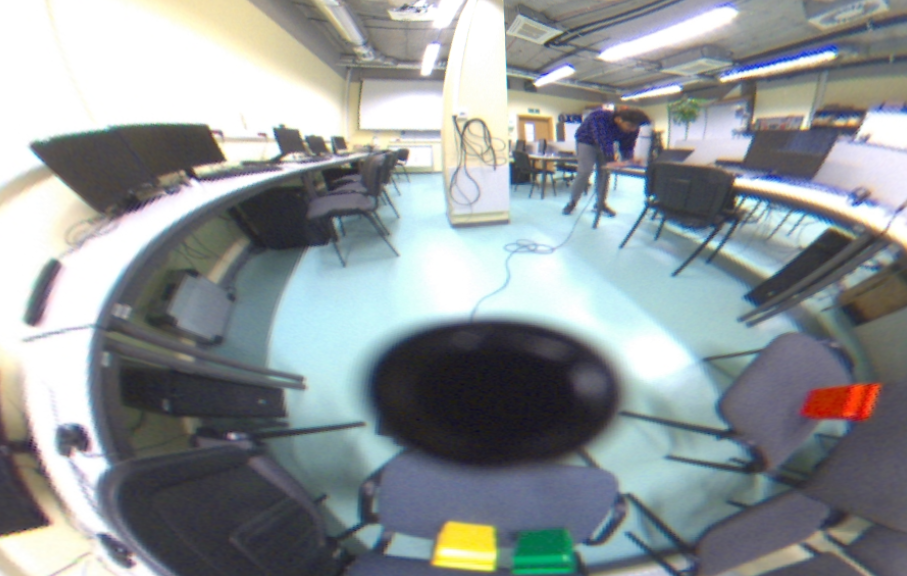
\includegraphics[scale=0.5]{Labbot&ele/q.png}
    \caption{Catadioptric Image- Distortion Removed(50 percent)}
    \label{fig:back} 
\end{figure}\

%%%%%%%%%%%%%%%%%%%%%%%%%%%%%%%%%%%%%%%%%%%%%%%%%%%%%%%%%%%
 \begin{figure}[H]
    \centering
    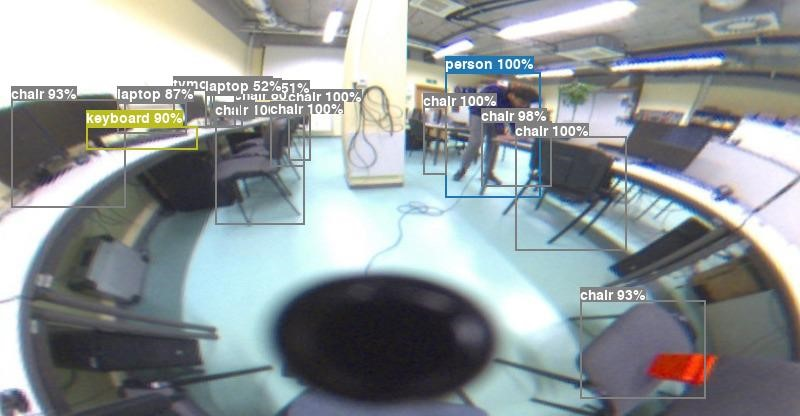
\includegraphics[scale=0.6]{Labbot&ele/m.jpg}
    \caption{YOLOv3 Object Recognition implementation in Lab321}
    \label{fig:back} 
\end{figure}\

 \begin{figure}[H]
    \centering
    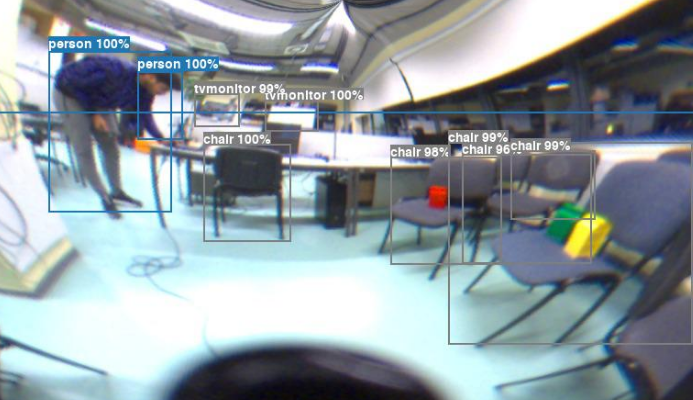
\includegraphics[scale=0.6]{Labbot&ele/test2.png}
    \caption{YOLOv3 Object Recognition implementation in Lab321}
    \label{fig:back} 
\end{figure}\
%%%%%%%%%%%%%%%%%%%%%%%%%%%%%%%%%%%%%%%%%%%%%%%%%%%%%%%%%%%%%%%%%%%%%%%%%%%%%%%%%%%%%%%%%%%%%%%%%%%%%%%%%
\subsection{TensorFlow Semantic Segmentation}
TensorFlow Semantic segmentation is an image segmentation technique that employs deep learning and TensorFlow, an open-source machine learning framework, to identify each pixel in an image based on a set of predetermined classes. Semantic segmentation is the process of assigning a class label to each pixel in an image in order to gain a more complete knowledge of the image's visual content.\newline
Deep learning architectures such as U-Net, DeepLab, and Mask R-CNN can be utilized for semantic segmentation. These architectures are primarily built on convolutional neural networks (CNNs) and are trained on large-scale datasets like COCO (Common Objects in Context) or PASCAL VOC, which contain images annotated at the pixel level.\newline
TensorFlow includes a suite of libraries and tools for training and deploying semantic segmentation models. For example, the TensorFlow Object Detection API offers a range of detection models, including ones for semantic segmentation, that can be readily trained and used in a TensorFlow environment. There are also additional libraries, such as TensorFlow-Slim, that make training and evaluating semantic segmentation models simple.\cite{zafar2018hands}\newline
Semantic segmentation is an important technique in computer vision with many applications, including self-driving automobiles, medical imaging, and robots. The TensorFlow framework and libraries make it simple to design and train semantic segmentation models, allowing for the development of increasingly accurate and sophisticated systems.
\subsection{SQL Flowchart to use the Google Colab platform to train a semantic segmentation model using the TensorFlow and Keras libraries}
\begin{lstlisting}
                    +-------+   +-------+   +----------+
        | Mount |-->| Install|-->| Import/  |
        | Drive |   | libs   |   | Setup    |
        +-------+   +-------+   +----------+
                     |            |
                     v            v
              +----------+    +----------+
              | Load     |    | Split    |
              | dataset  |    | dataset  |
              +----------+    +----------+
                     |            |
                     v            v
              +----------+    +----------+
              | Load img/|    | Create   |
              | mask     |    | model    |
              +----------+    +----------+
                     |            |
                     v            v
              +----------+    +----------+
              | Compile  |    | Set up   |
              | model    |    | callbacks|
              +----------+    +----------+
                     |            |
                     v            v
              +----------+    +----------+
              | Print    |    | Train    |
              | summary  |    | model    |
              +----------+    +----------+
                     |            |
                     v            v
              +----------+    +----------+
              | Predict  |    |  -       |
              | masks    |    |  -       |
              +----------+    +----------+

\end{lstlisting}

\begin{algorithm}[H]
\caption{Segmentation Model Training}
\label{alg:segmentation_model_training}
\begin{algorithmic}[1]
\Procedure{Segmentation Model Training}{}
\State Mount Google Drive to access dataset
\State Install libraries: "segmentation-models", "tf-semantic-segmentation"
\State Import libraries and set framework for segmentation model to TensorFlow/Keras
\State Load dataset from Google Drive
\State Split dataset into training and validation sets
\State Load random image from training set, display and print shapes
\State Create ERFNet model, compile with Adam optimizer, binary crossentropy loss, accuracy metrics
\State Set up Tensorboard callbacks, save best model
\State Print model summary and train on training set, evaluate with validation set
\State Use trained model to make predictions on training and validation sets, threshold to create binary masks
\EndProcedure
\end{algorithmic}
\end{algorithm}
 

%%%%%%%%%%%%%%%%%%%%%%%%%%%%%%%%%%%%%%%%%%%%%%%%%%%%%%%%%%%%%%%%%%%%%%%%%%%%%%%%%%%%%%%%%%%%%%%%%%%%%%%%%
\begin{figure}[H]
    \centering
    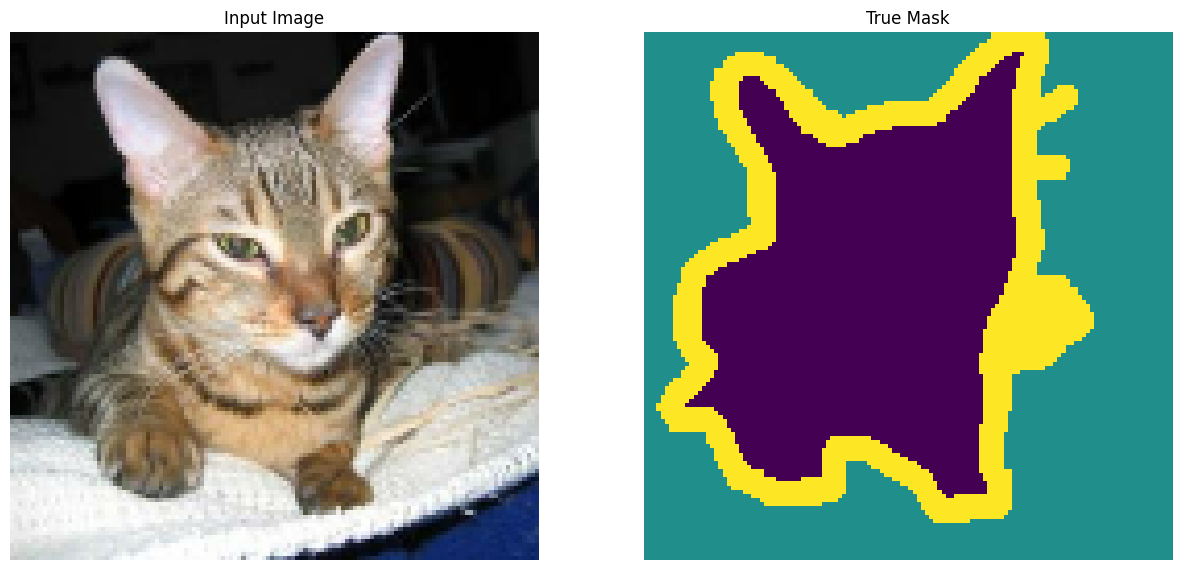
\includegraphics[scale=0.4]{Labbot&ele/16.png}
    \caption{TF-Segmentation Example}.
    \label{fig:print} 
\end{figure}\


%%%%%%%%%%%%%%%%%%%%%%%%%%%%%%%%%%%%%%%%%%%%%%%%%%%%%%%%%%%%%%%%%%%%%%%%%%%%%%%%%%%%%%%%%%%%%%%%%%%%%%%%%
\begin{figure}[H]
    \centering
    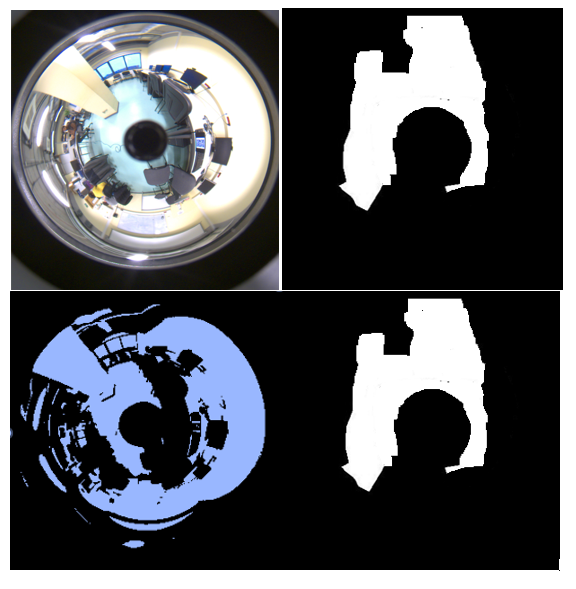
\includegraphics[scale=0.9]{Labbot&ele/tf-segment.png}
    \caption{TF-Segmentation-An example of a segmentation result: a correctly marked free space on right}.
    \label{fig:print} 
\end{figure}

\section{Obstacle Avoidance Method}
This functionality can be implemented in a variety of ways - as with other work on the LabBot robot, the YOLO convolutional network will do well for this, which performs the task of realtime object detection, though its use is associated with a disadvantage - such models recognize the types of objects that have been learned, which necessitates training the network on a wide range of obstacles. There is a high risk of a collision if the robot moves towards an object that does not belong to any of the classes on which the neural network (implemented on it) has not been trained.\newline
With this in mind, the focus of the navigation system's architecture was on a more universal approach, based not on the object detection problem, but on binary semantic segmentation.\cite{li2020vision}
\subsection{Navigation Algorithm}

\begin{algorithm}
\caption{Robot Navigation Algorithm}
\begin{algorithmic}[1]
\Procedure{Navigate}{}
\State Determine the target sector
\State Turn to a sector that faces the target directly or indirectly depending on obstacles
\While{true}
\State Rotate until the difference between the current angle and the center of the target sector is below 0.1 radians
\State Correct omni wheel alignment
\If{current sector is on the list of available sectors with a minimum of 50 percent free space}
\State Move forward
\Else
\State Stop the robot
\State Select a new driving direction
\EndIf
\EndWhile
\EndProcedure
\end{algorithmic}
\end{algorithm}
\newpage
\subsection{Semantic Segmentation and Ground Truth Mask}
The goal of semantic segmentation is to split an image into uniform sections that correspond to the things or places seen on it and are representations of different classes. To distinguish which class a certain pixel belongs, all pixels in the image are labeled (e.g., in numerical form) (each pixel of a given object receives the same label).
\newline
The neural network utilized will eventually have two classes at its output: open space and the rest of the environment, which will be handled as a general impediment. We can discuss the example of binary semantic segmentation (or the task of background subtraction).
The graphic below juxtaposes two photos from the robot's camera with examples of the truth masks that were meant to be achieved.
\begin{figure}[H]
    \centering
    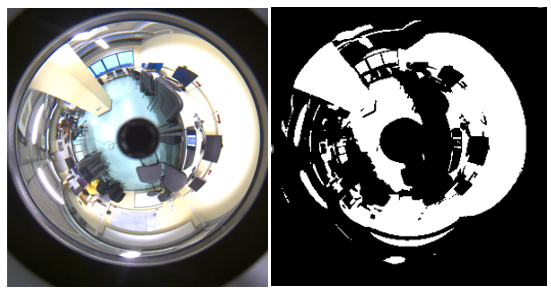
\includegraphics[scale=1]{Labbot&ele/tf2.png}
    \caption{Semantic omnidirectional image segmentation}.
    \label{fig:print} 
\end{figure}

\subsection{CVAT}
CVAT (Computer Vision Annotation Tool) is an open-source annotation tool created by Intel Corporation that is used to create and manage image and video annotation projects. It is intended to make the annotation process more efficient and time-efficient by offering an intuitive interface for creating and altering object bounding boxes, polygon masks, keypoints, and other annotation types.
\newline
It provides a web-based interface through which users can browse and annotate photos and videos, as well as collaborate on the same annotation project. It can recognise objects, do semantic segmentation, instance segmentation, and detect keypoints, among other things. It also lets users import and export annotation data in a variety of formats, including COCO, VOC, and YOLO.
\newline
It also includes annotation enhancements such as automatic annotation suggestions, annotation quality management, and annotation statistics. It also has an annotation quality control system that allows users to examine, accept, or reject annotations submitted by other users.
\newline
It is a sophisticated annotation tool that can assist computer vision researchers and engineers in fast and easily creating high-quality annotation datasets. It's widely used in industry and research, and because it's open source, it's simple to customize and combine with other tools and systems.
For data labeling, the free and interactive web environment CVAT (Computer Vision Annotation Tool) was employed. Before you could use it, you had to register, create a dataset tagging task on your account, and name and color all identifiable classes. It was possible back then to use previously prepared images in .png format as the basis for learning the neural network.Data might now be marked up from that point forward. 



\subsection{Data Augmentation and Neural Architecture}
Data augmentation is a technique for increasing the size of a dataset artificially by applying various alterations to the current data. Techniques such as flipping, rotating, cropping, and scaling photos, adding noise, and adjusting brightness and contrast are examples of this. Data augmentation is useful in training deep learning models, especially in the field of computer vision, where large-scale annotated datasets are often scarce. By applying these adjustments to current data, the model can learn to detect objects and patterns in a variety of orientations, lighting situations, and scales, improving its robustness and generalization abilities.

Data augmentation can be used in the context of obstacle avoidance to mimic various scenarios and surroundings that a robot or autonomous vehicle may experience.
By rotating and flipping photos of barriers, for example, the model can learn to detect them from various angles and orientations. Similarly, by adding noise to photos or adjusting their brightness and contrast, the model may learn to spot obstacles in a variety of lighting settings.
Obstacle avoidance is also aided by neural networks. In obstacle avoidance, Convolutional Neural Networks (CNNs) are extensively utilized. CNNs are capable of detecting objects and barriers in pictures and videos and may be trained to do so. Recurrent Neural Networks (RNNs) are also employed for obstacle avoidance. RNNs are useful for comprehending data sequences, such as a series of photos from a camera.They can be used to predict the robot's future step, which can assist the robot in avoiding obstacles.

Another neural design that is extensively utilized in semantic segmentation is the Fully Convolutional Networks (FCN), which can predict the class of each pixel in an image. It may be used to forecast obstacles in images, which can help robots and autonomous vehicles navigate and avoid obstacles in their environment.

Overall, data augmentation and neural architectures play essential roles in obstacle avoidance.
\subsection{Steps for Data augmentation algorithms}
The following steps apply several data augmentation algorithms to a series of input images and masks before saving the augmented images and masks to a specified directory.

\begin{algorithm}
\caption{Augment Images and Masks}
\label{alg:augment}
\begin{algorithmic}[1]
\State Check if the directories for storing the augmented images and masks exist. If they do not, create them.
\State Initialize two lists \textit{images} and \textit{masks} to store the paths of the images and masks respectively
\State Populate \textit{images} by appending the path of each image in the \textit{SCREEN-PATH} directory, and \textit{masks} by appending the path of each mask in the \textit{MASK-PATH} directory.
\State Use the \textit{albumentations} library to define a set of augmentations that will be applied to the images and masks
\State Define a variable \textit{images-to-generate} to specify the number of augmented images needed
\For {$i \gets 1$ to \textit{images-to-generate}}
\State Select a random image and its corresponding mask from \textit{images} and \textit{masks} respectively
\State Read the selected image and mask
\State Apply the augmentations defined earlier to the image and mask
\State Save the augmented image and mask in the directories
\EndFor
\end{algorithmic}
\end{algorithm}

This is a procedure to augment images and masks. First, the code checks if the directories for storing the augmented images and masks exist. If they don't, it creates them. Next, it initializes two lists, 'images' and 'masks', to store the paths of the images and masks that need to be augmented. The 'images' list is populated by appending the path of each image in the 'SCREEN-PATH' directory, and the 'masks' list is populated by appending the path of each mask in the 'MASK-PATH' directory. Then, the 'albumentations' library is used to define a set of augmentations that will be applied to the images and masks. A variable 'images-to-generate' is defined to specify the number of augmented images needed. A for loop is used to iterate 'images-to-generate' number of times. In each iteration, a random image and its corresponding mask is selected from the 'images' and 'masks' list, respectively. The selected image and mask are read and the augmentations defined earlier are applied to them. Finally, the augmented image and mask are saved in the directories.








\chapter{Evaluation and Conclusions}
\section{Results of the efficient navigation}
Originally, it was intended to develop a comprehensive model capable of navigating both inside and outside the M321 laboratory. The experiments began by collecting data in the laboratory and teaching the ERFNet.
Attempts to produce outcomes that allow for effective navigation resulted in the first data set consisted of 500 photos recorded solely in artificial light because of bad weather.
 Parameters of the learning process:
 \begin{itemize}
     \item 500 images with a division of 70\% training, 30\% validation
     \item  Training duration: 80 epochs
     \item Batch size = 10
     \item Optimizer = Adam
     \item initialized learning rate = 0.001
     \item loss function was Binary Crossentropy
 \end{itemize}
 The outcome of the Segmentation was correct but there was so many areas which was not detected correctly after the attempt.First I thought it is because of bad weather but later after research I came to know a small data-set might be an issue.The results were satisfactory, with the free space masks avoiding the impediments in the new photos. However, after performing real-time tests, it was decided to train the model for another 100 epochs since, as feared, when the illumination changed significantly, the neural network did not perceive a free spot where the light reflections were.
 
 \begin{figure}[H]
    \centering
    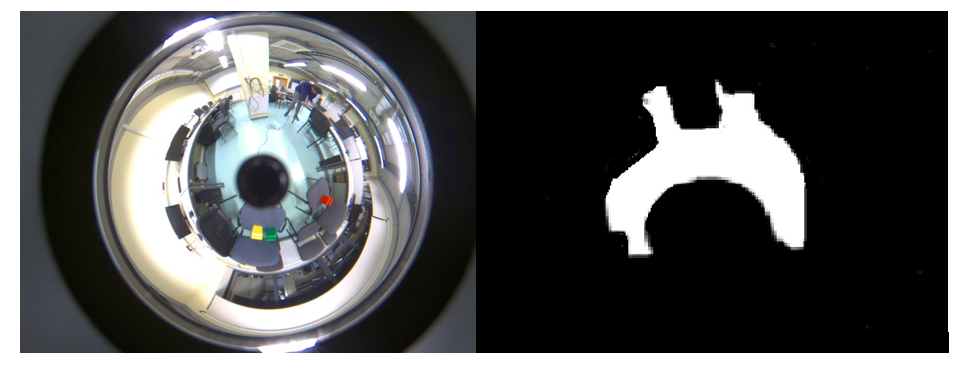
\includegraphics[scale=0.6]{Labbot&ele/conclusion2.png}
    \caption{Segmentation result: some correctly detected, some incorrectly }
    \label{fig:print} 
\end{figure}

 \begin{figure}[H]
    \centering
    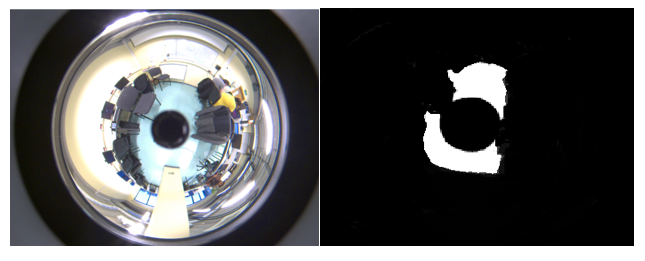
\includegraphics[scale=0.9]{Labbot&ele/w3.png}
    \caption{Segmentation result: some correctly detected, some incorrectly }
    \label{fig:print} 
\end{figure}

 \begin{figure}[H]
    \centering
    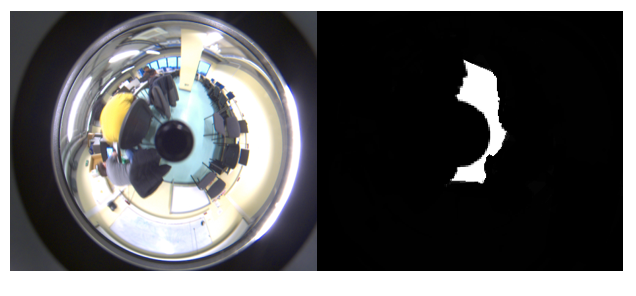
\includegraphics[scale=0.9]{Labbot&ele/w4.png}
    \caption{Segmentation result: some correctly detected, some incorrectly }
    \label{fig:print} 
\end{figure}

\subsection{Obstacle Avoidance Testing}
Initially,The working environment for the labBot was including only artificial light. Due to bad weather condition, Testing was not done during the sunlight hours, but using artificial lights which plays similar role during image sensing.
In the beginning, attempts were made to test the robot on a single wall of chairs, tables, or other objects that had been used to create an obstacle course for the dataset. It turns out that while cardboard boxes were typically viewed as open space, armchairs and tables had trouble with the area between their legs. The fact that they turned dark after the robot got close enough to cast a shadow on them may have contributed to this. The second flaw was that LabBot was approaching the objects it was avoiding too closely.This led to collisions in the majority of situations, especially when combined with forecast efficiency .\newline
The obstacle was successfully avoided for the first time after this adjustment. However, the robot did not move as fluidly as the algorithm's theoretical premise indicated. The obstacle was successfully detected, but because the LabBot was close to it, it occasionally took unnecessary turns in an effort to move in the right direction.\newline
In the end for confirmation , I choose a designated area with some obstacles for the confirmation of obstacle avoidance.It was deemed adequate proof of the implemented control's successful operation.

  \begin{figure}[H]
    \centering
    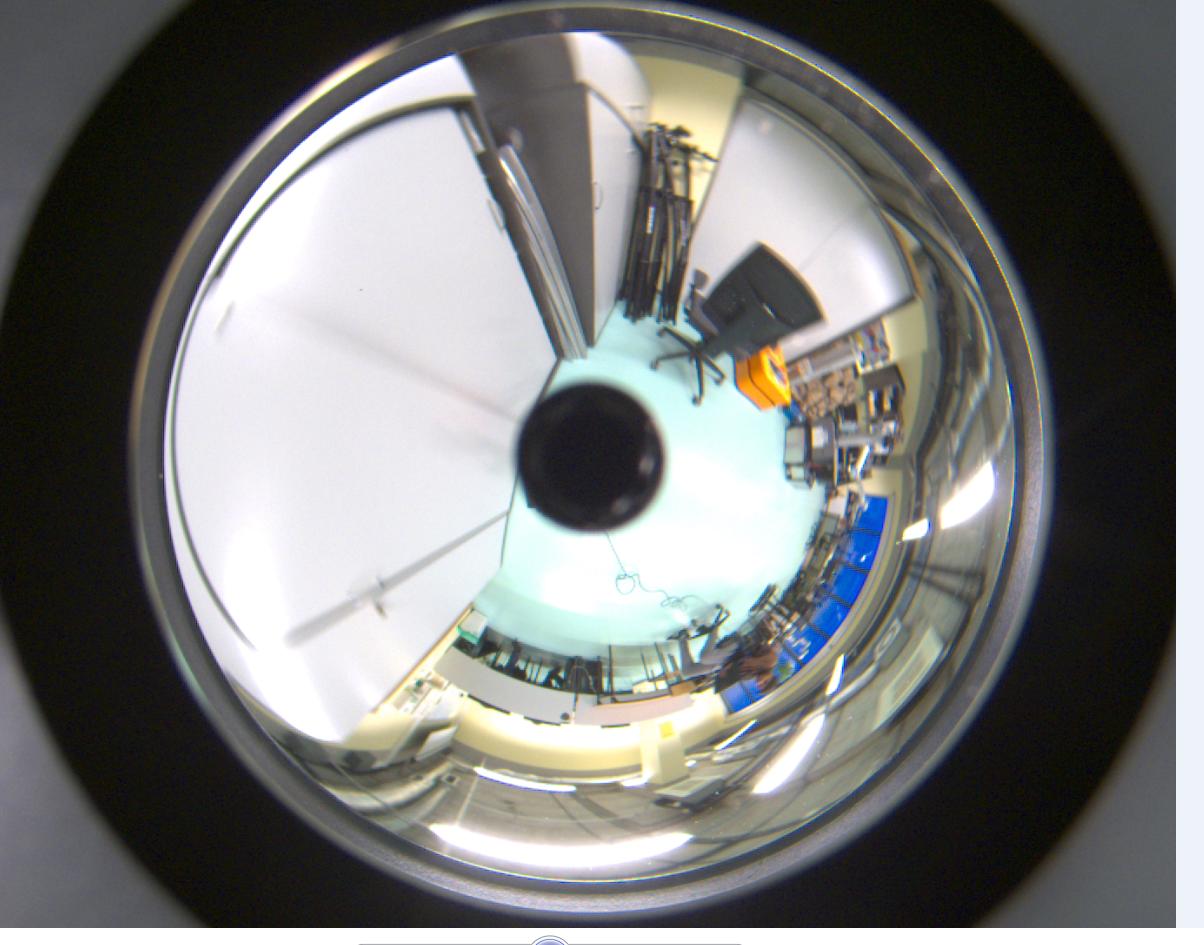
\includegraphics[scale=0.3]{Labbot&ele/obs1.png}
    \caption{Sample image from the navigation process}
    \label{fig:print} 
\end{figure}
  \begin{figure}[H]
    \centering
    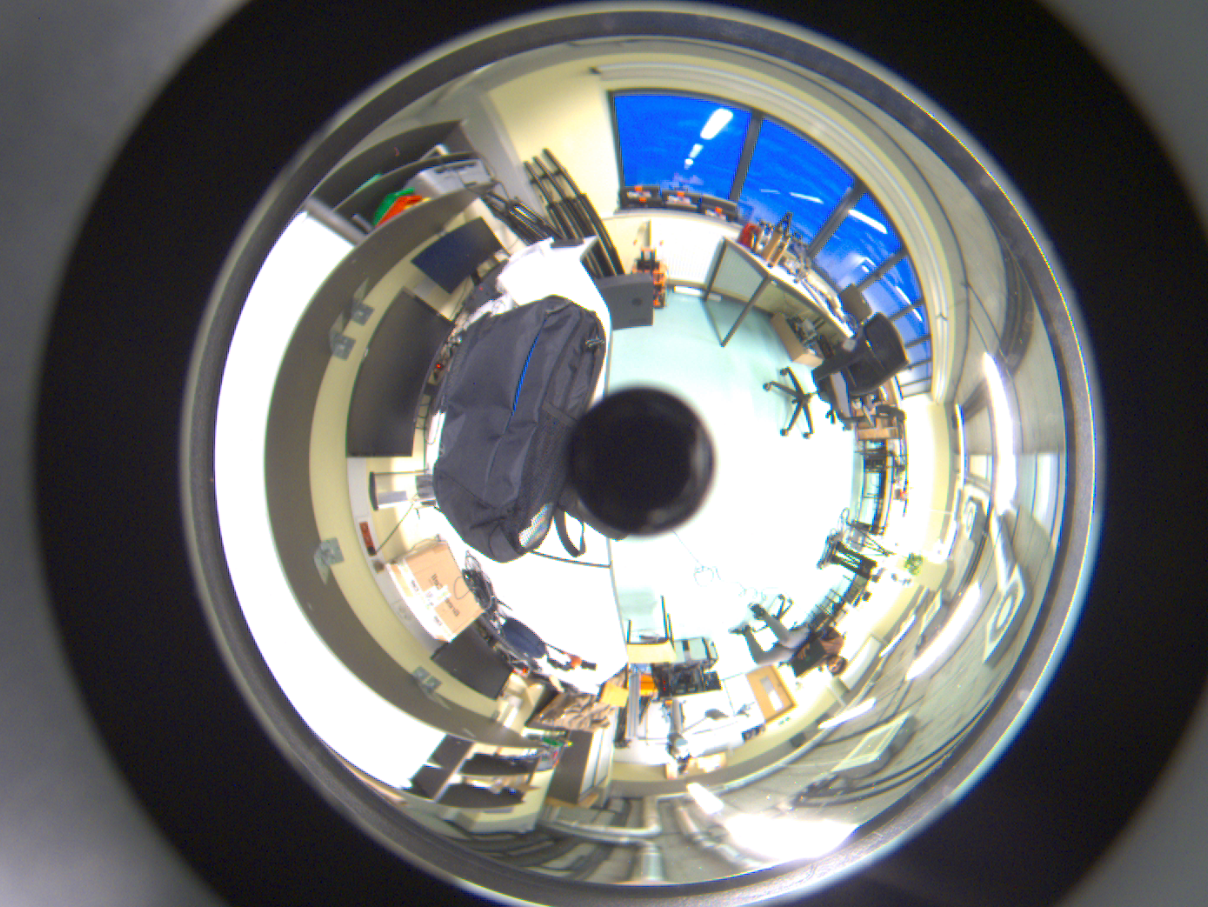
\includegraphics[scale=0.3]{Labbot&ele/obs2.png}
    \caption{Sample image from the navigation process}
    \label{fig:print} 
\end{figure}


\subsubsection{Final attempt- No change in weather condition}
In the next attempt ,I decided to increase the data-set to 1000 images with following parameters.
\begin{itemize}
     \item 1000 images with a division of 80\% training, 20\% validation
     \item Training duration: 100 epochs
     \item Batch size = 10
     \item Optimizer = Adam
     \item initialized learning rate = 0.001
     \item loss function was Binary Crossentropy
 \end{itemize}

 \begin{figure}[H]
    \centering
    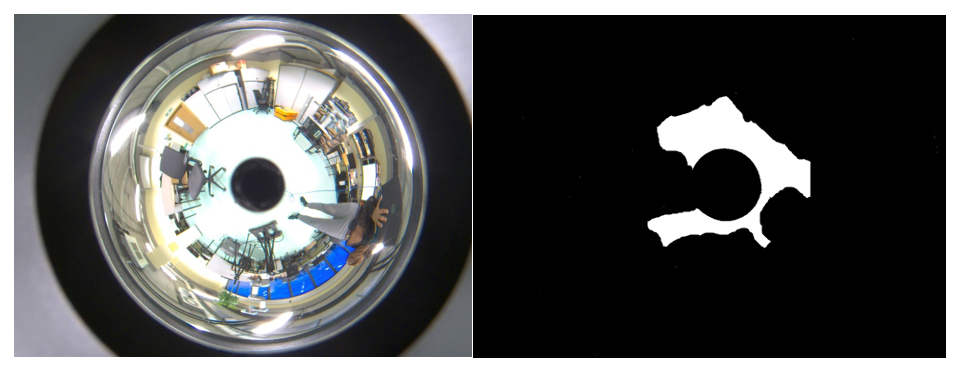
\includegraphics[scale=0.6]{Labbot&ele/conclusion1.png}
    \caption{Segmentation result: a correctly marked free space }
    \label{fig:print} 
\end{figure}

 \begin{figure}[H]
    \centering
    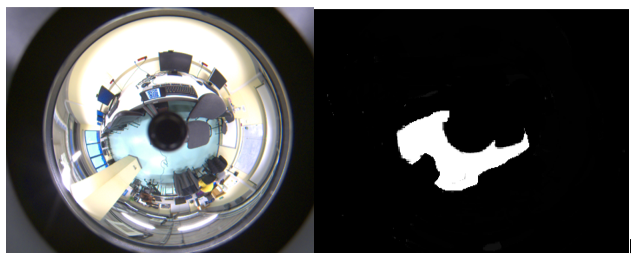
\includegraphics[scale=0.9]{Labbot&ele/w5.png}
    \caption{Segmentation result: a correctly marked free space }
    \label{fig:print} 
\end{figure}

 \begin{figure}[H]
    \centering
    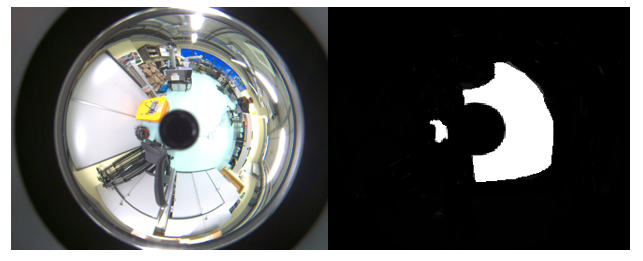
\includegraphics[scale=0.9]{Labbot&ele/w6.png}
    \caption{Segmentation result: a correctly marked free space }
    \label{fig:print} 
\end{figure}



\section{Conclusions}
The thesis "Catadioptric Vision System for the LabBot Mobile Robot" aims to create and test a catadioptric vision system for a mobile robot. Installation of a catadioptric sensor on the mobile robot, calibration of the camera sensor, development of a ROS node for image acquisition, implementation of an obstacle avoidance method, and implementation of an object recognition function are among the tasks done in this thesis.\newline
The installation of the catadioptric sensor on the mobile robot required mechanical, electrical, and assembly work, all of which were completed successfully. Calibration of the camera sensor was critical to ensuring that the sensor captured high-quality catadioptric images. The ROS node's implementation and image acquisition from the catadioptric camera was successful.\newline
Based on the omnidirectional images acquired by the sensor, an obstacle avoidance method was developed and proven to be successful at avoiding obstacles. The object identification technology added to the robot aided in better comprehension of the environment.
The system was tested and reviewed in many scenarios and confirmed to work as predicted. Overall, the thesis demonstrated the viability and efficacy of adopting a catadioptric vision system for a mobile robot.\newline
The incorporation of a catadioptric sensor in a mobile robot, as well as obstacle avoidance and object recognition, can significantly increase the performance and functionality of mobile robots in a variety of applications such as surveillance, self-driving automobiles, robotics, drones, and surveying.\newline
    
\bibliographystyle{plain}
\bibliography{references}


\end{document}